\subsection{Correlations in the signal region}
We present the correlations among variables in the signal region in
the figures \ref{fig:corrMatrix_SR} and
\ref{fig:correlations_SR_drbjets_S} and \ref{fig:correlations_SR_drbjets_BG}.

%\begin{center}
\begin{figure}[!htb]%hbpt?        
\centering

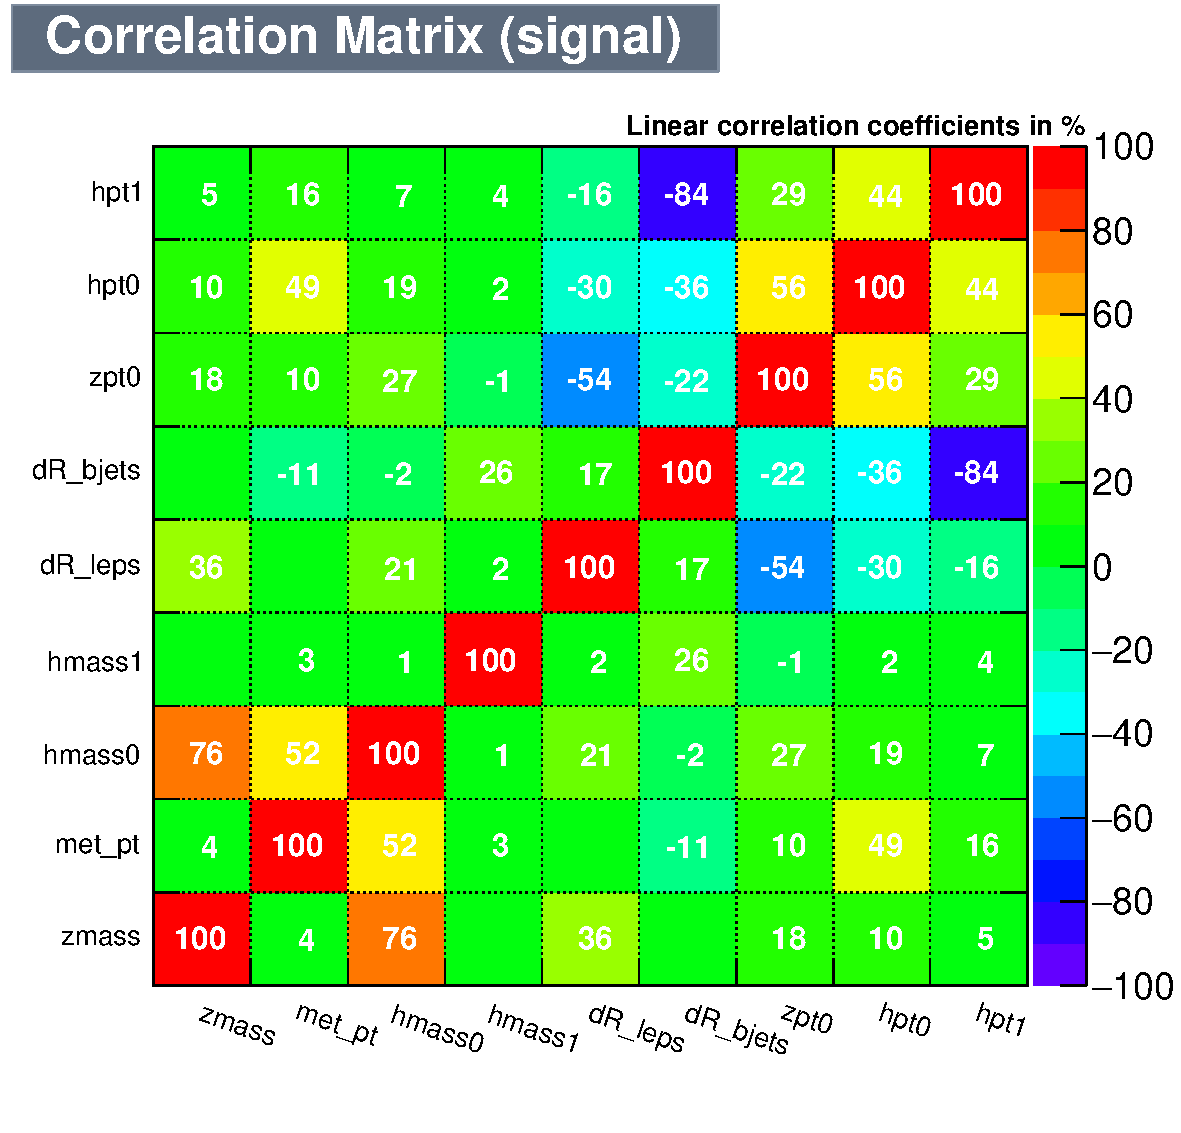
\includegraphics[width=0.65\textwidth]{figures/SR/dataset/plots/CorrelationMatrixS.pdf}
\bigbreak
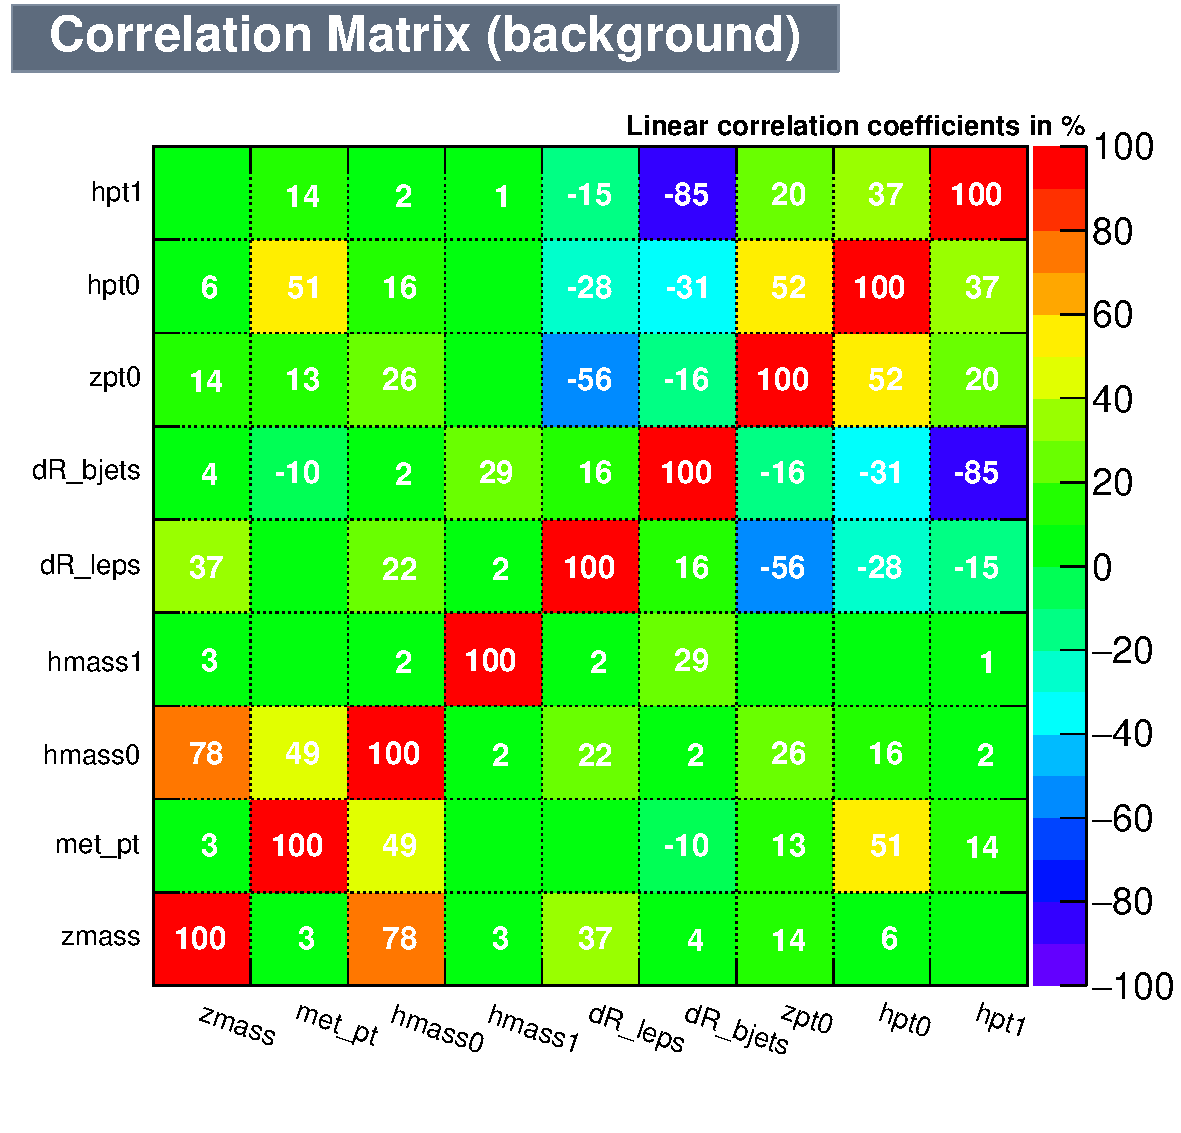
\includegraphics[width=0.65\textwidth]{figures/SR/dataset/plots/CorrelationMatrixB.pdf}
%% 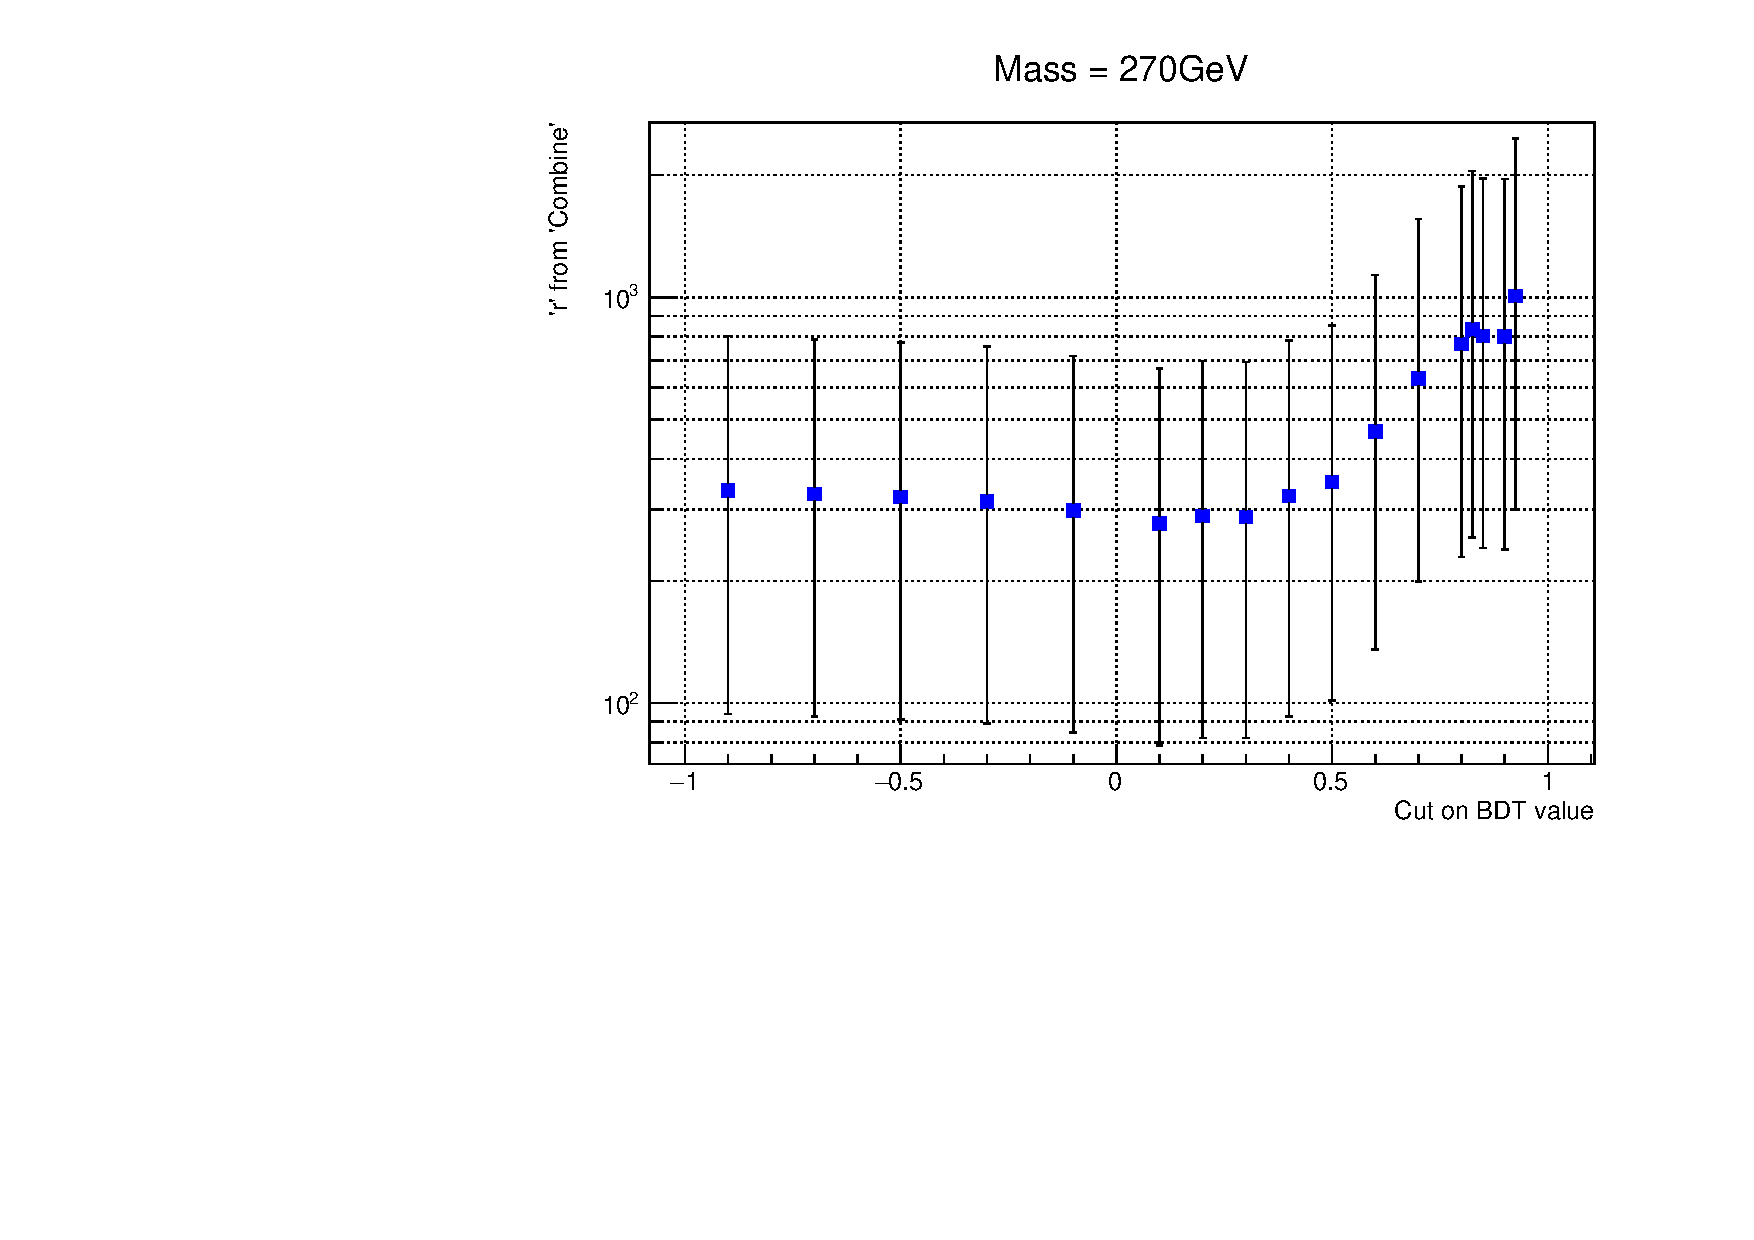
\includegraphics[width=0.5\textwidth, height=0.2\textheight,  keepaspectratio]{figures/eles_bdt_vs_r/gr_limits__270GeV.pdf}
%% 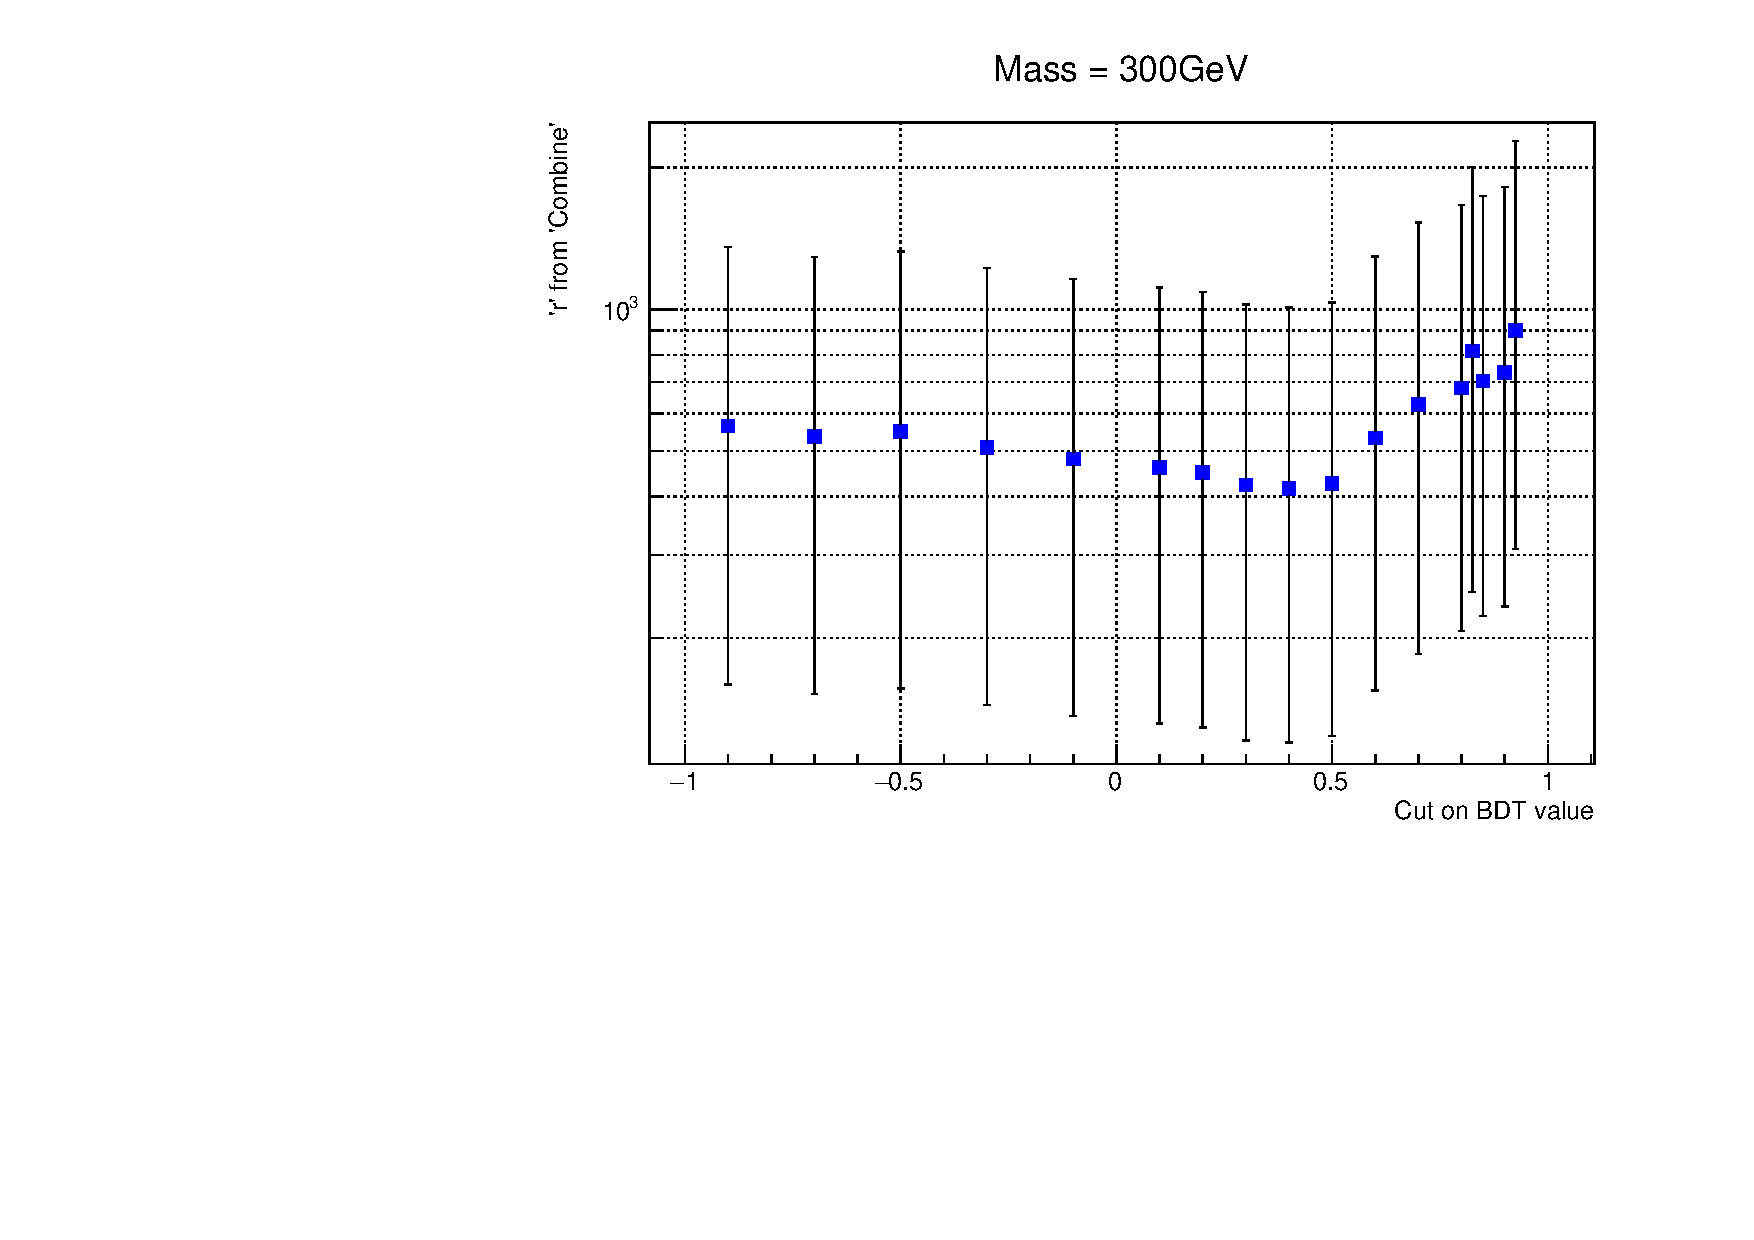
\includegraphics[width=0.5\textwidth, height=0.2\textheight,  keepaspectratio]{figures/eles_bdt_vs_r/gr_limits__300GeV.pdf}
%% 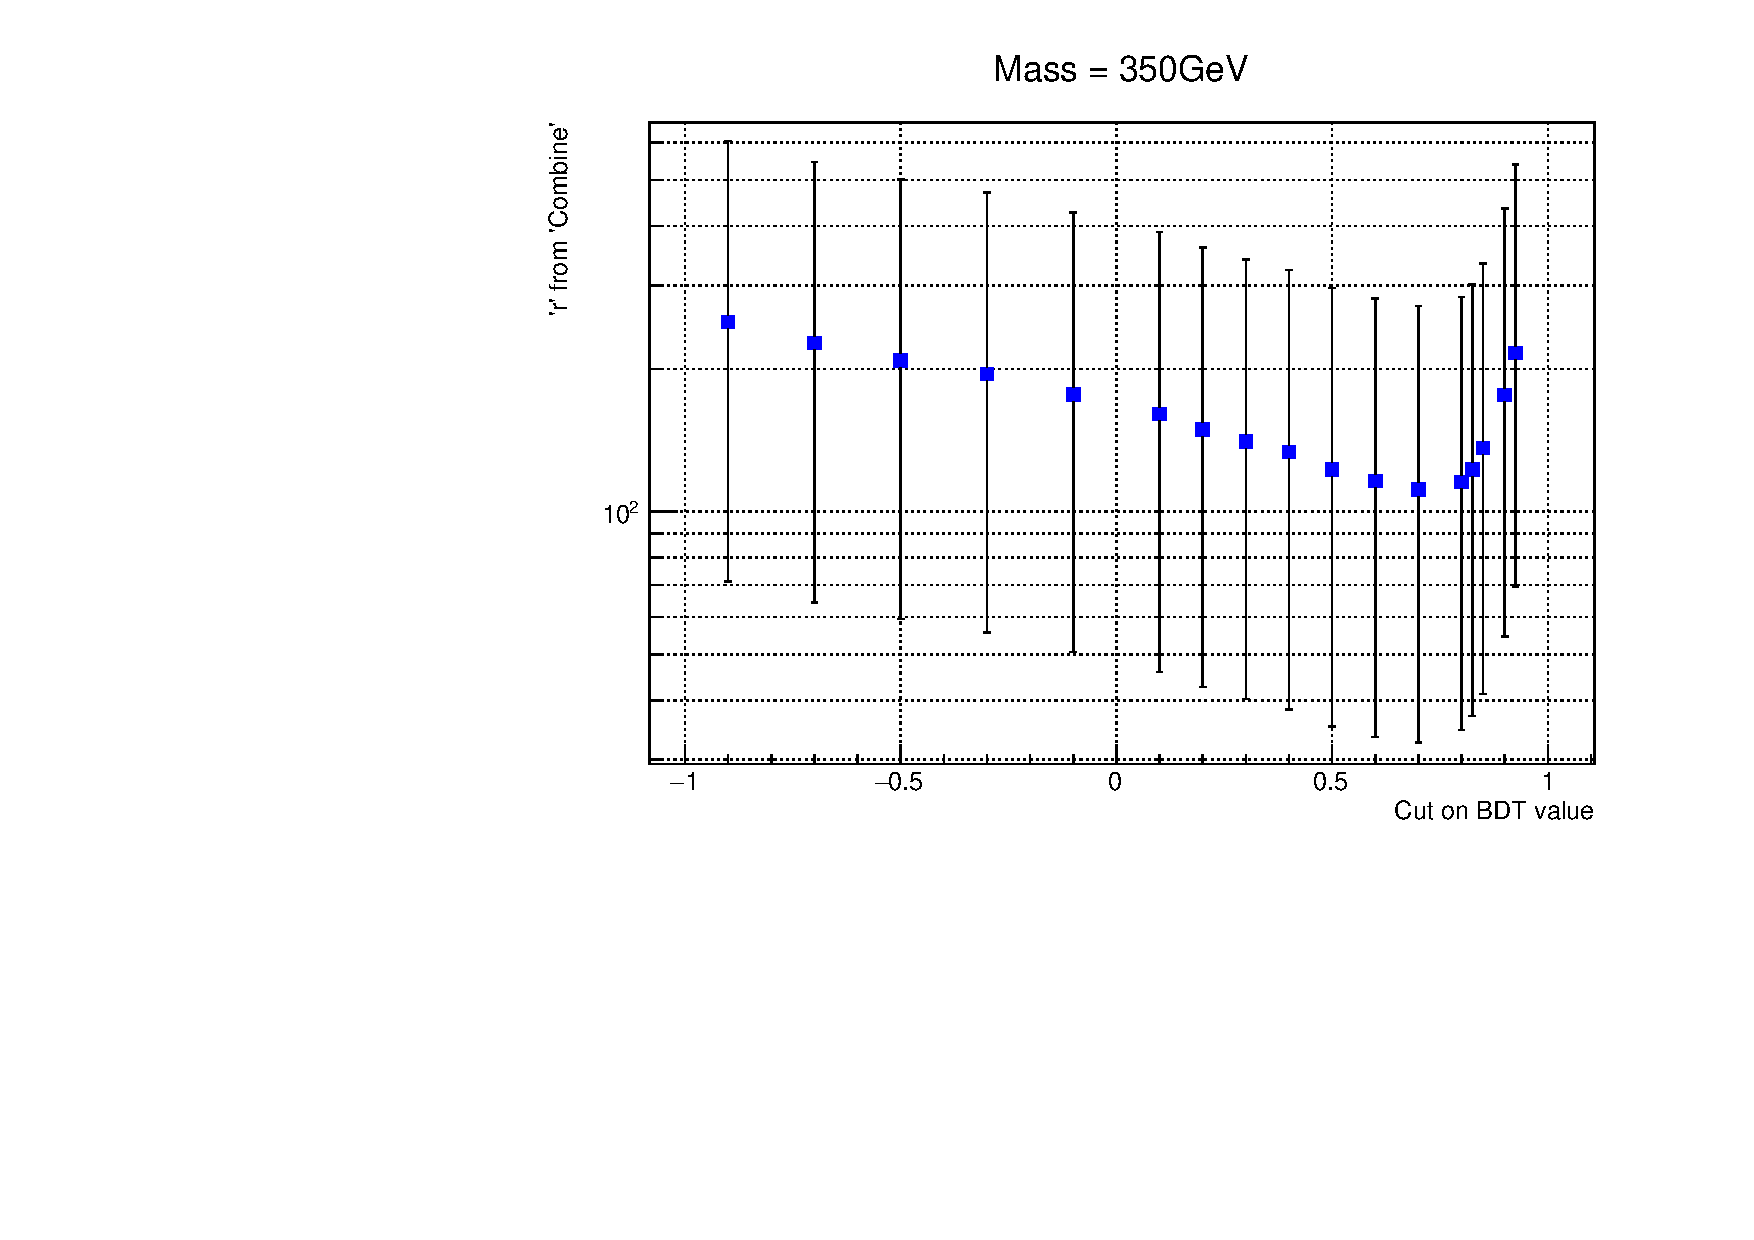
\includegraphics[width=0.5\textwidth, height=0.2\textheight,  keepaspectratio]{figures/eles_bdt_vs_r/gr_limits__350GeV.pdf}
%% 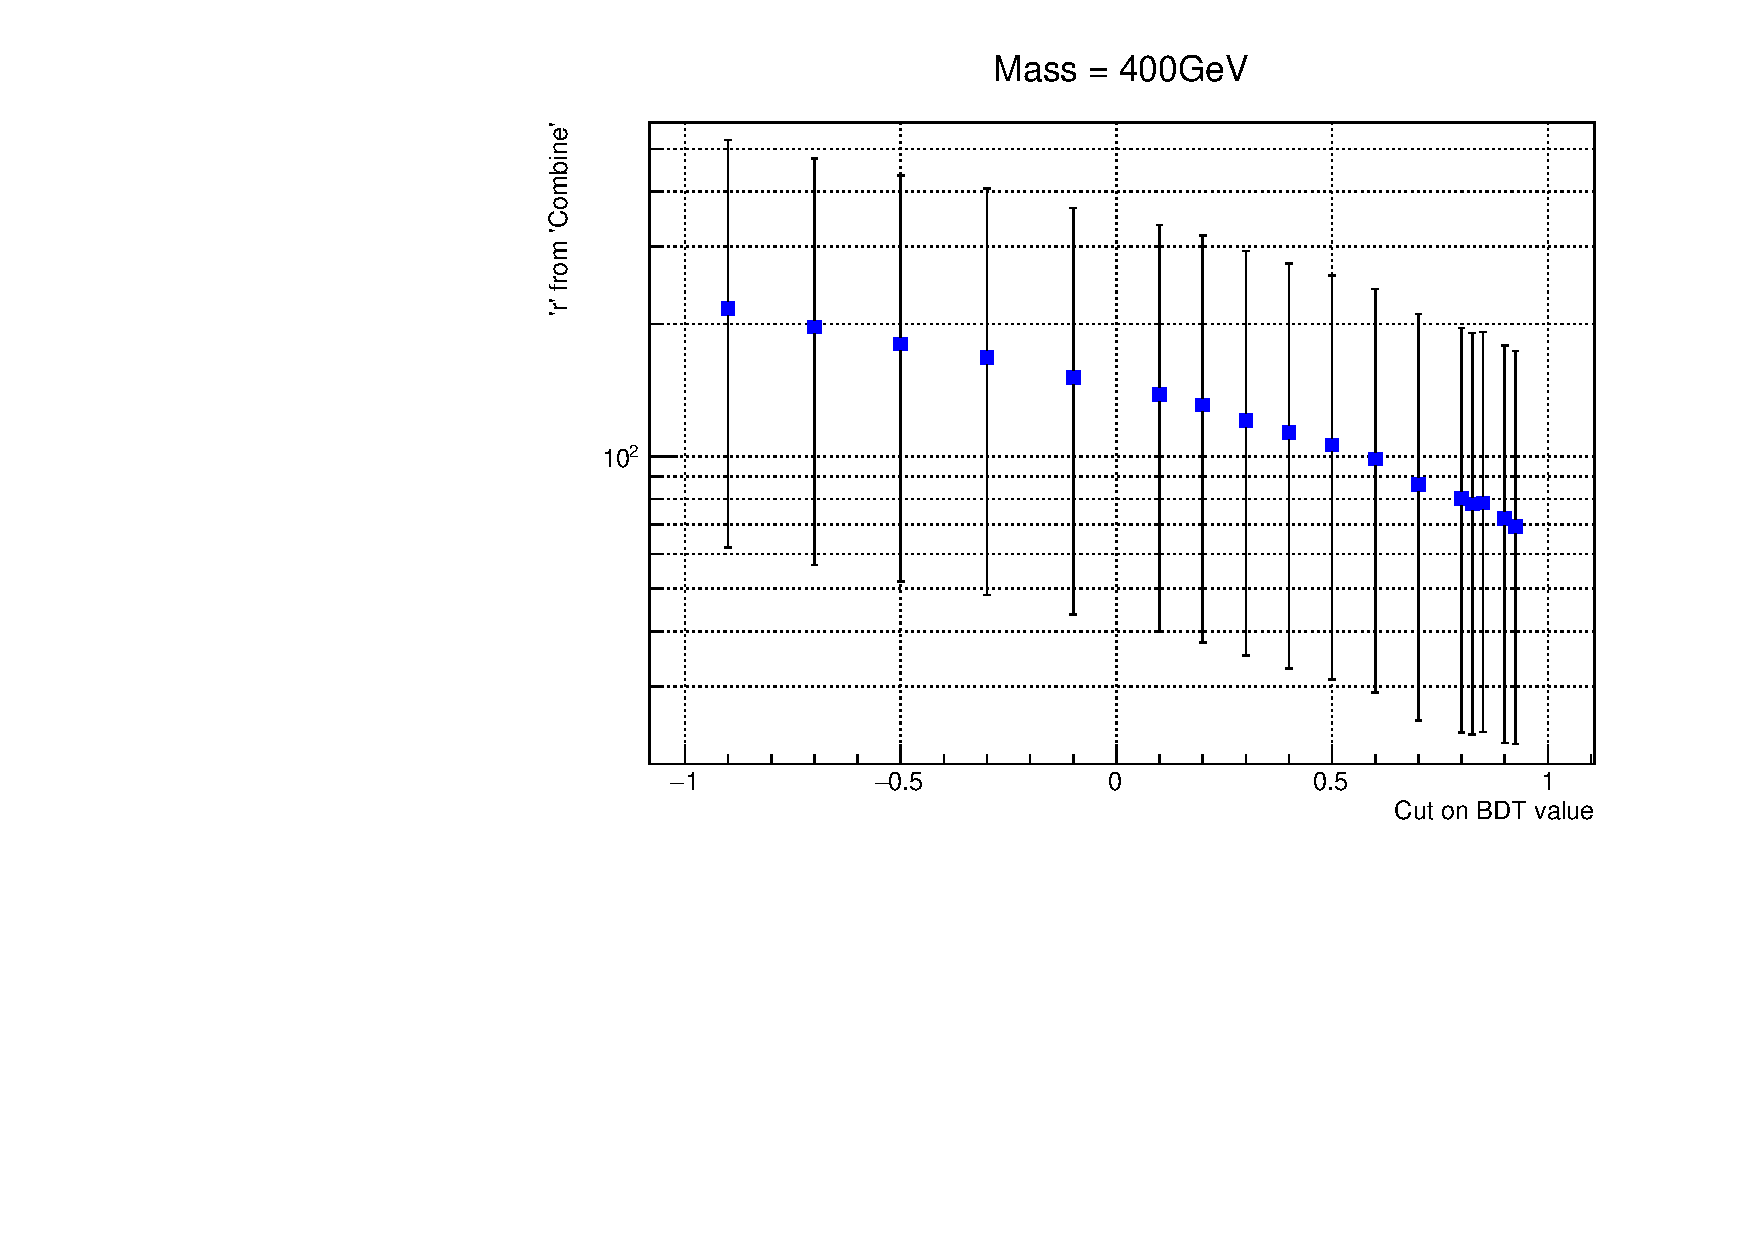
\includegraphics[width=0.5\textwidth, height=0.2\textheight,  keepaspectratio]{figures/eles_bdt_vs_r/gr_limits__400GeV.pdf}
%% 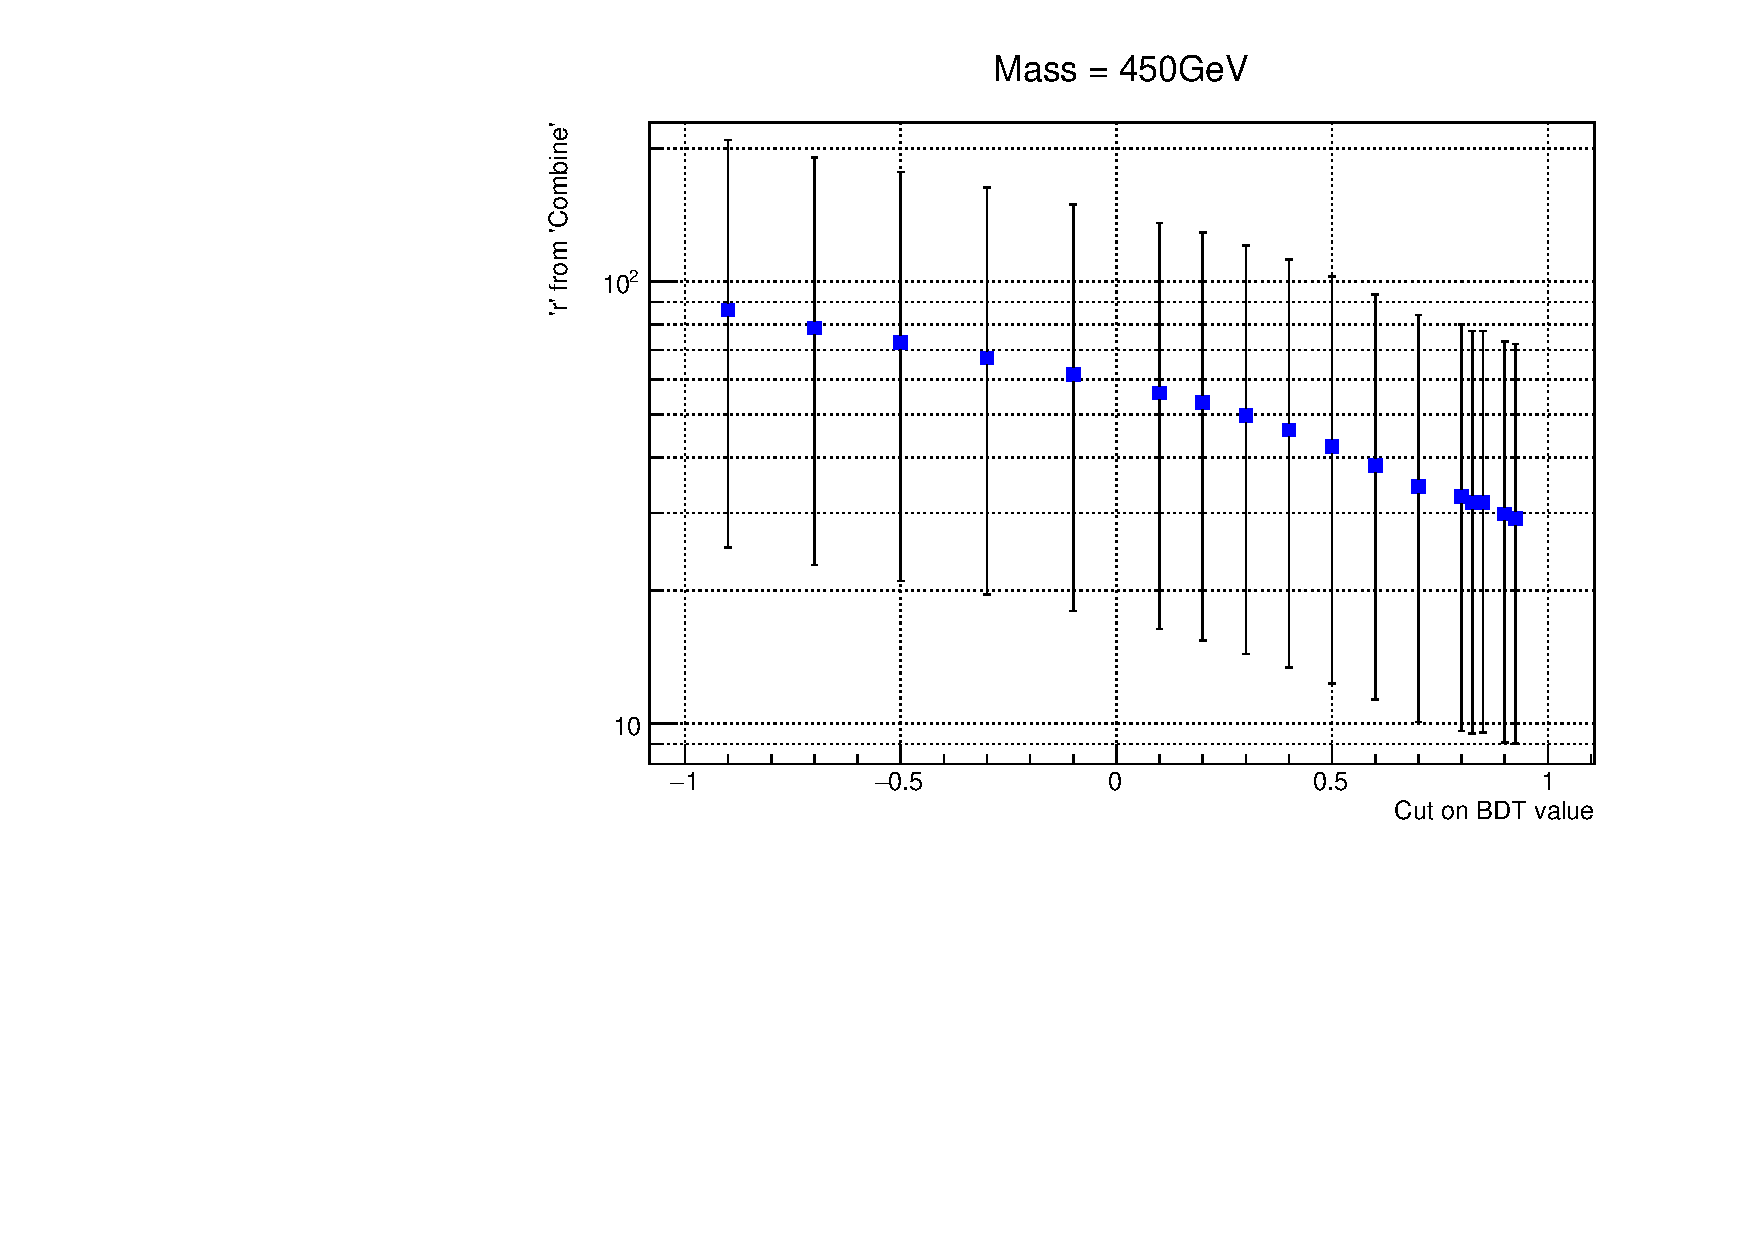
\includegraphics[width=0.5\textwidth, height=0.2\textheight, keepaspectratio]{figures/eles_bdt_vs_r/gr_limits__450GeV.pdf}
%% 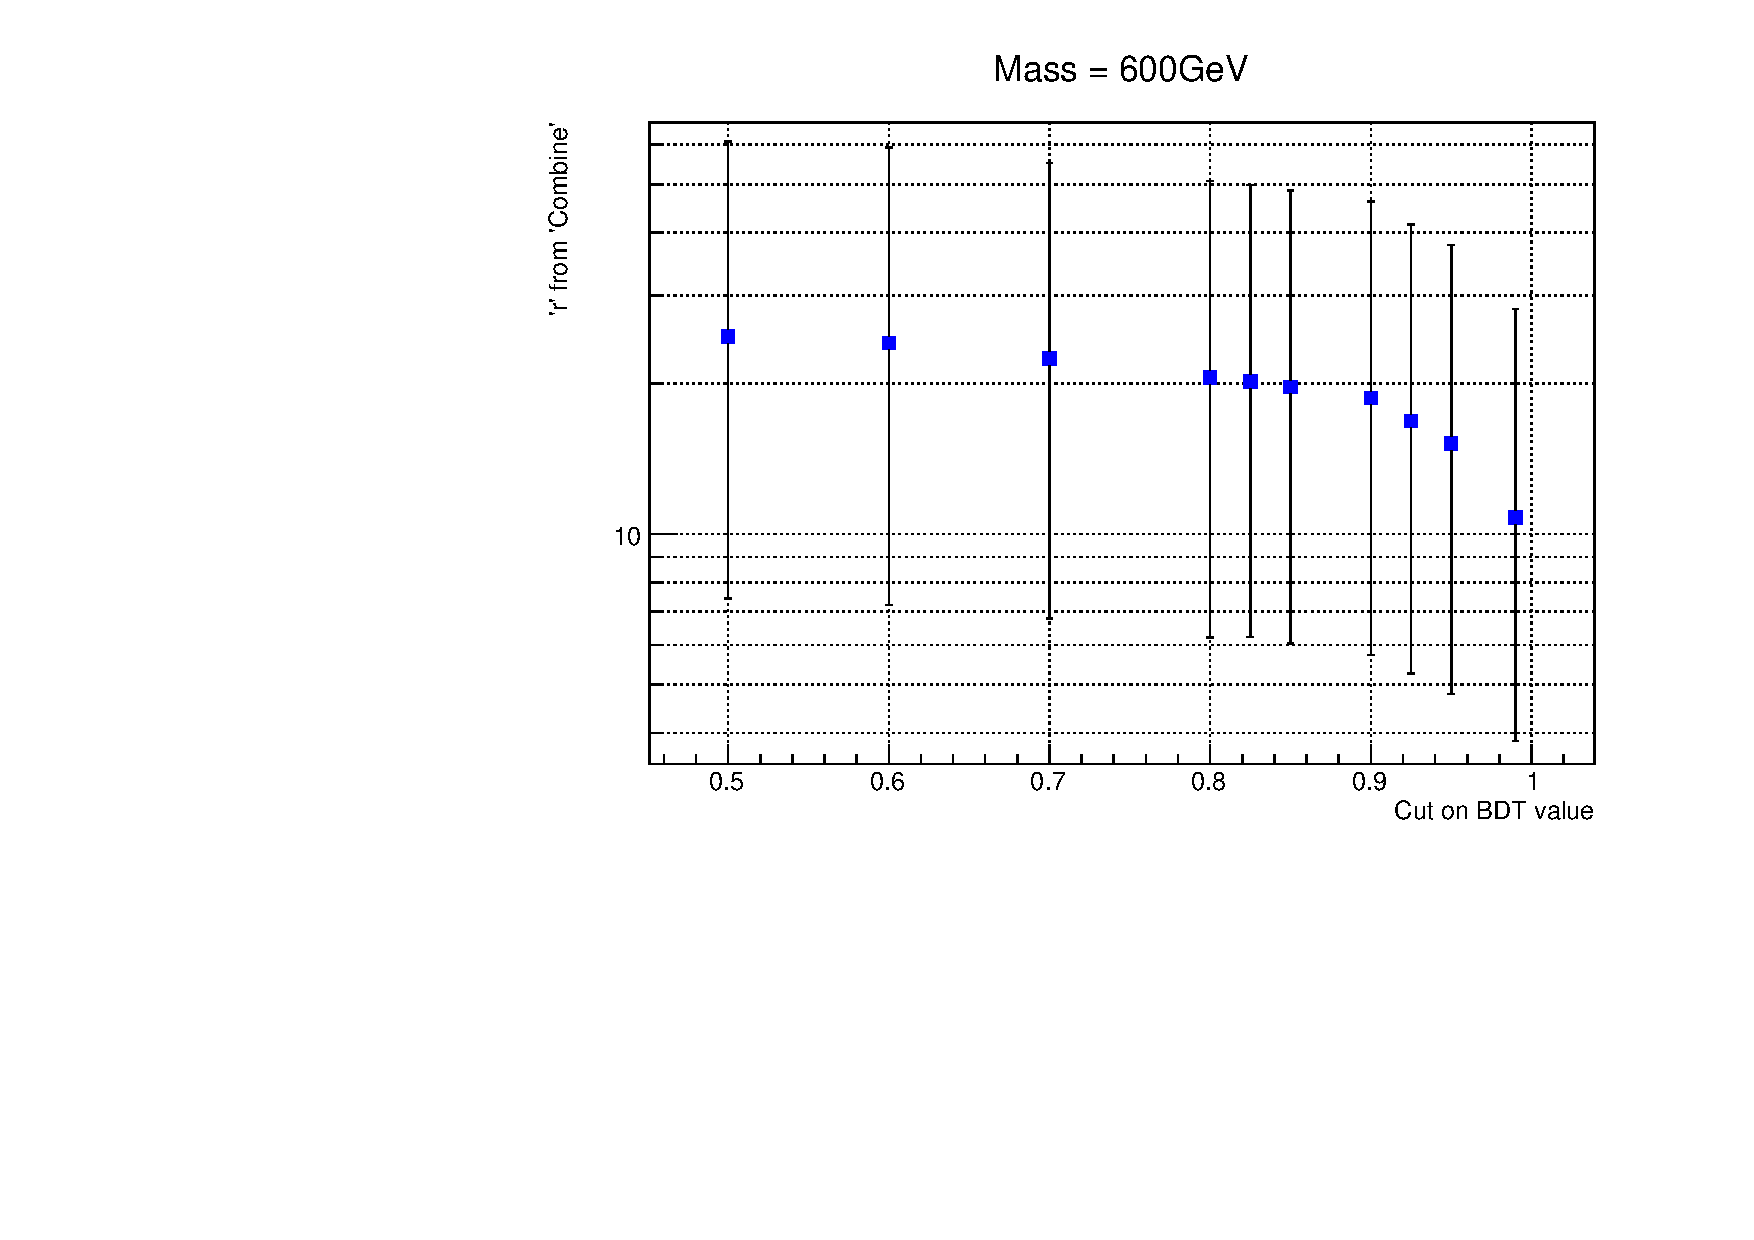
\includegraphics[width=0.5\textwidth, height=0.2\textheight, keepaspectratio]{figures/eles_bdt_vs_r/gr_limits__600GeV.pdf}
%% 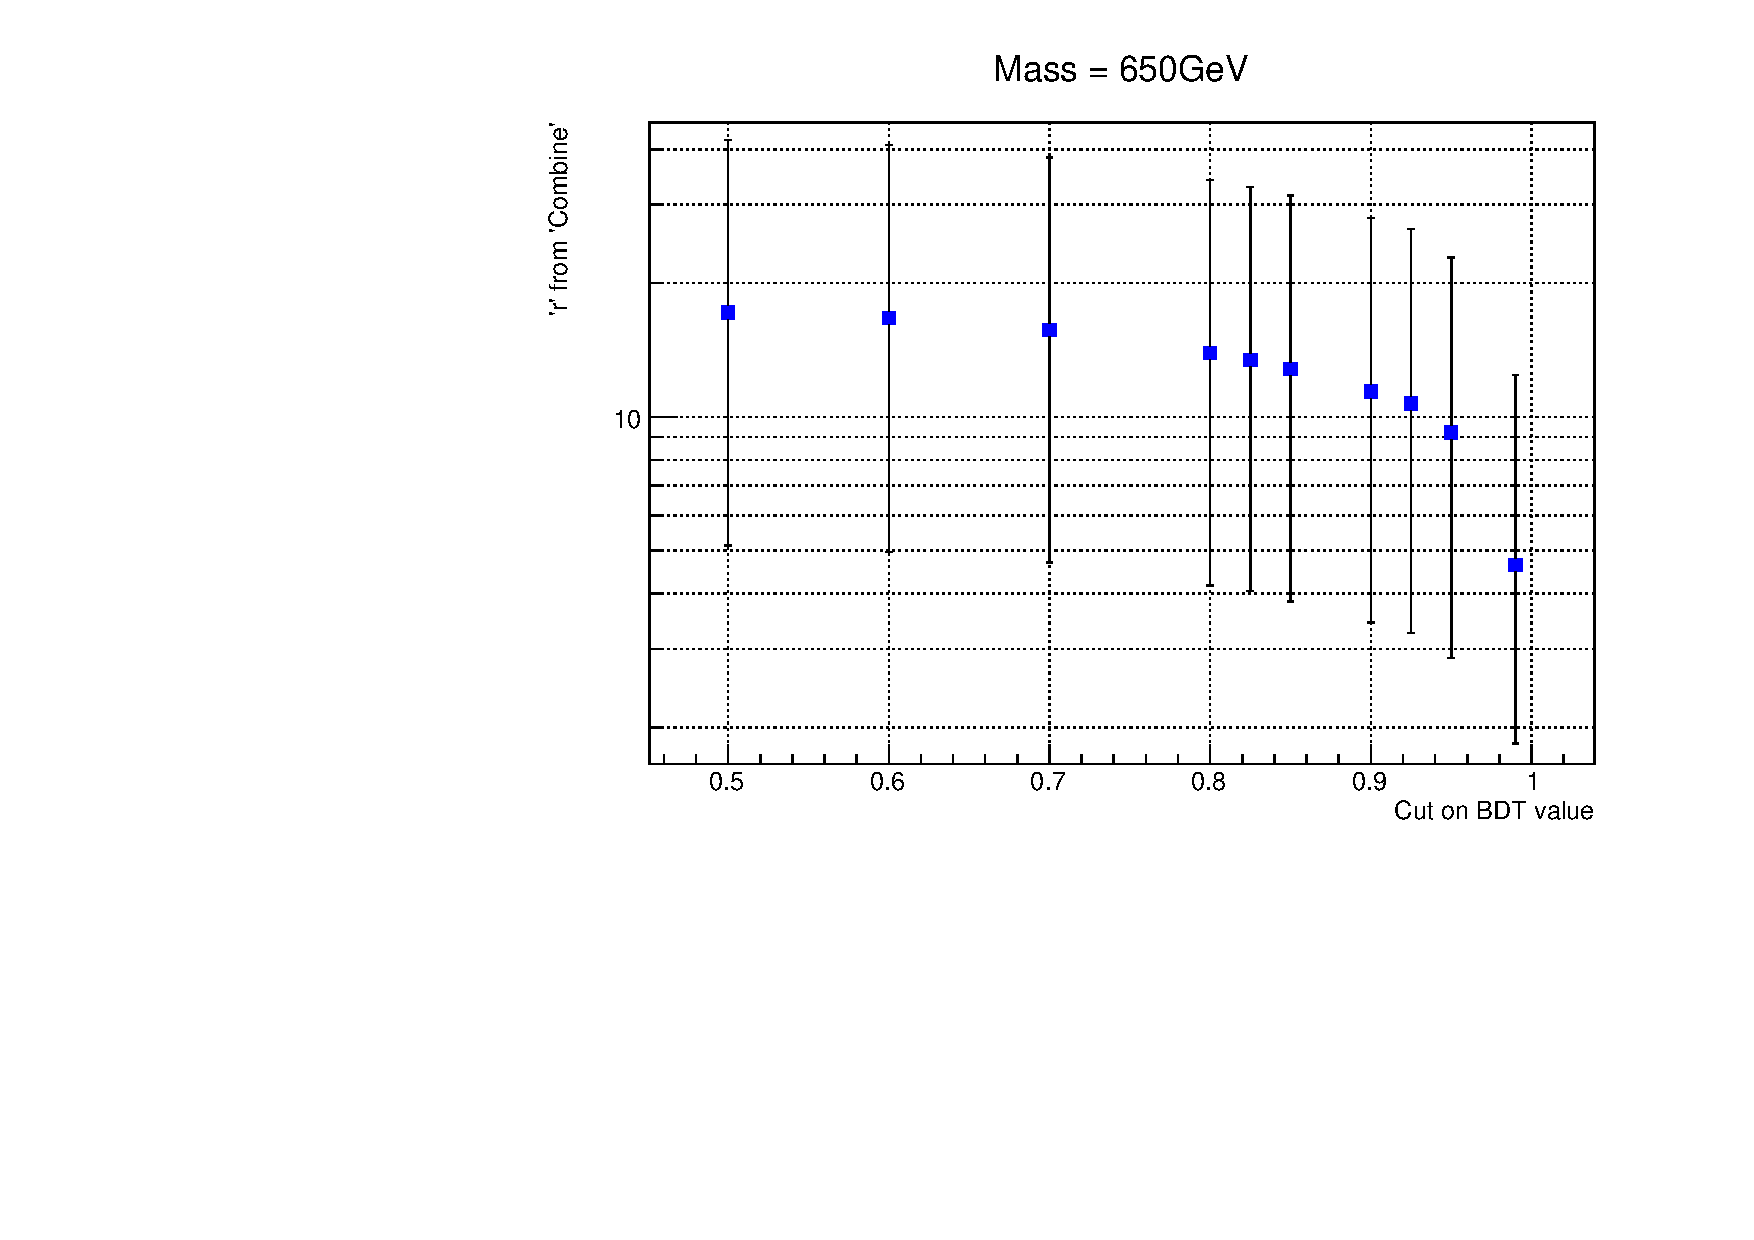
\includegraphics[width=0.5\textwidth, height=0.2\textheight, keepaspectratio]{figures/eles_bdt_vs_r/gr_limits__650GeV.pdf}
%% 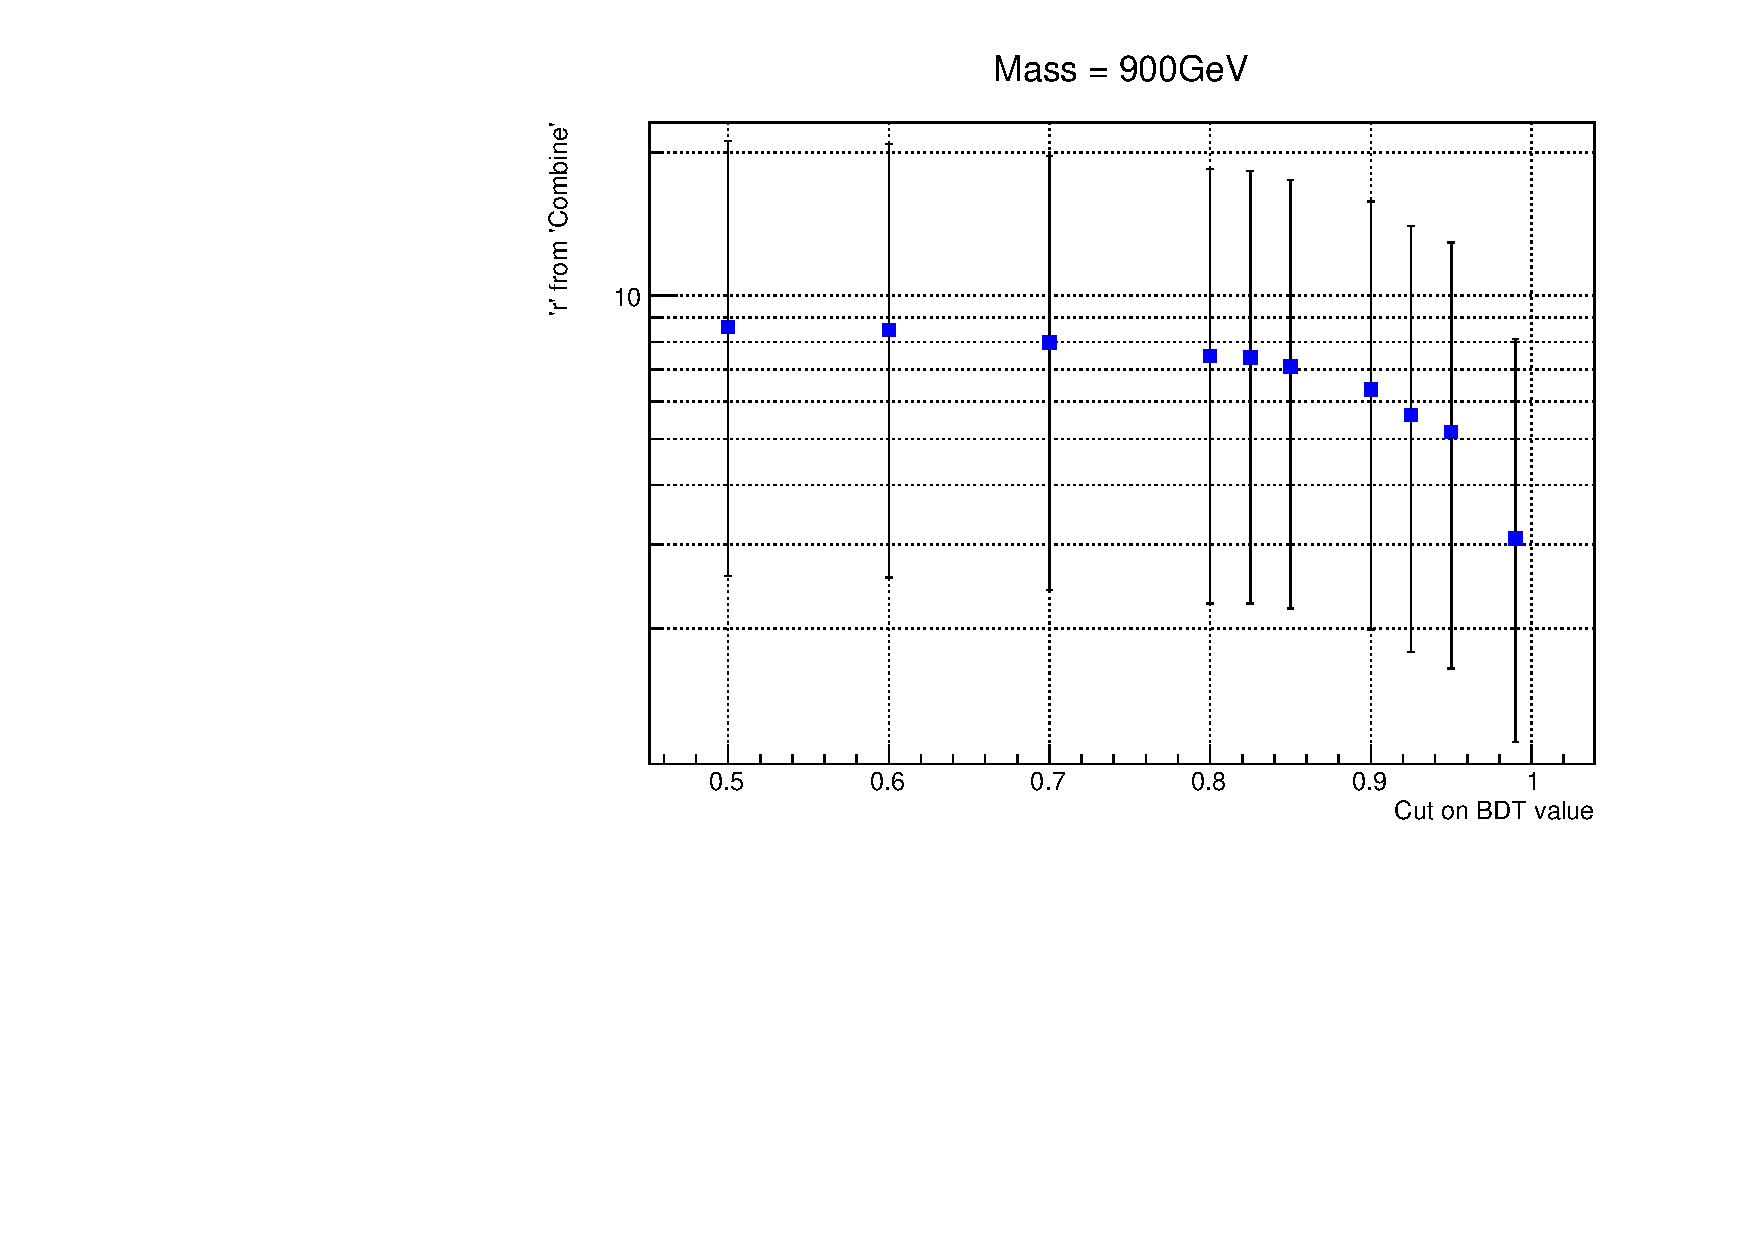
\includegraphics[width=0.5\textwidth, height=0.2\textheight, keepaspectratio]{figures/eles_bdt_vs_r/gr_limits__900GeV.pdf}
%% \hspace{1.9cm}
%% 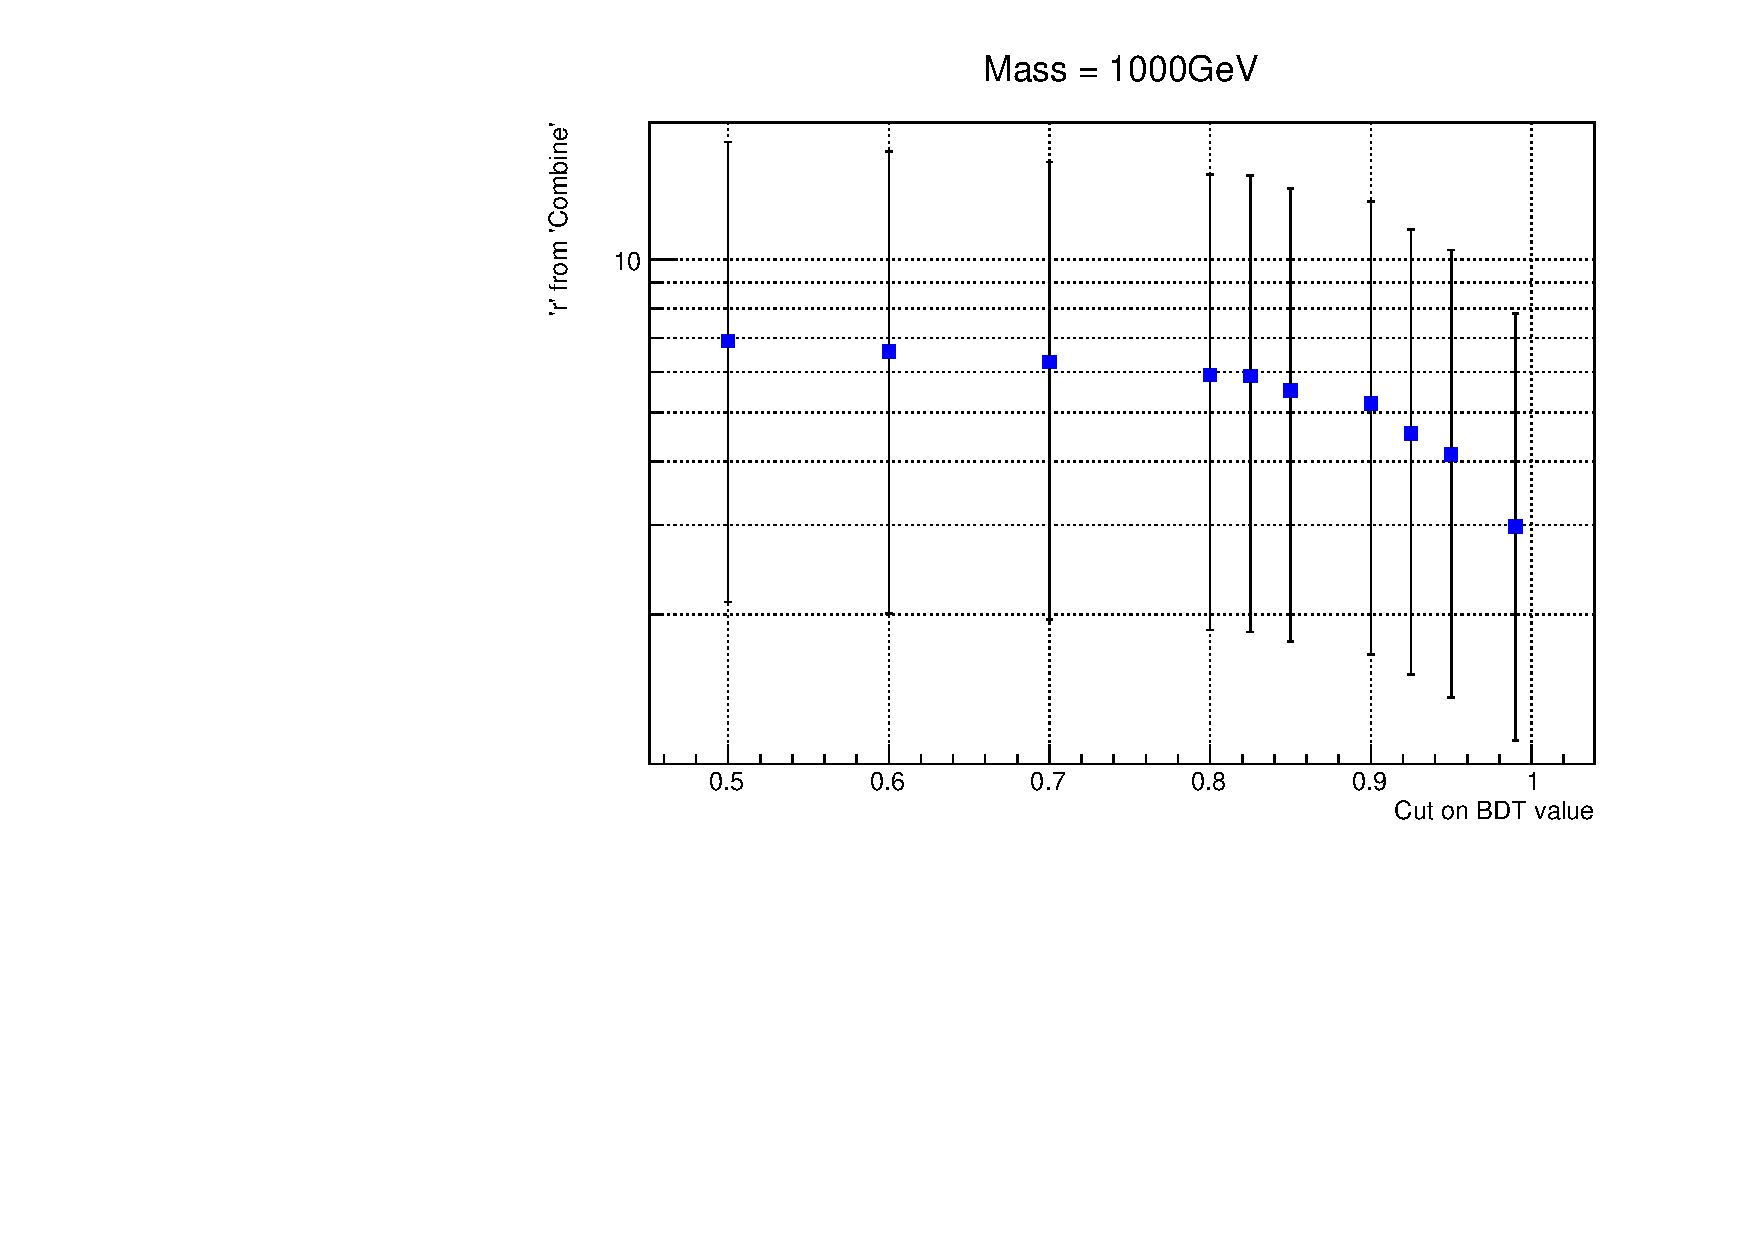
\includegraphics[width=0.5\textwidth, height=0.2\textheight, keepaspectratio]{figures/eles_bdt_vs_r/gr_limits__1000GeV.pdf}
\caption{ Correlation matrices for the signal and background (mix of DY and TT) in the signal region, in the names of few variables the index '1' refers to bb and the index '0' refers to ZZ}
\label{fig:corrMatrix_SR}                                                       
\end{figure}
%\end{center}





\begin{figure}[!htb]%hbpt?        
\centering
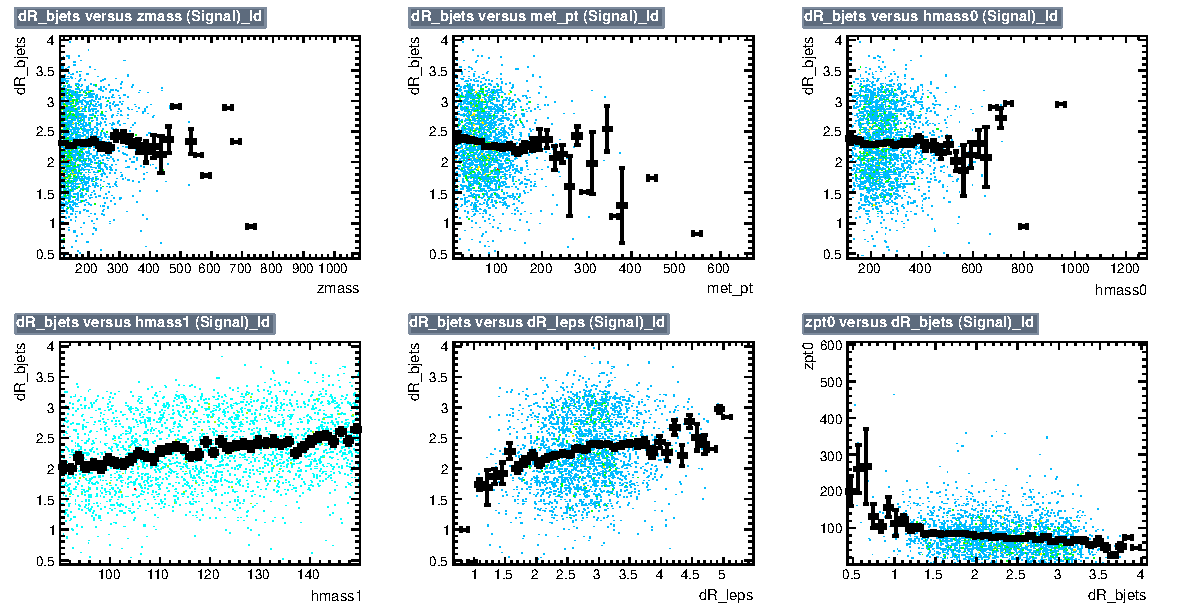
\includegraphics[width=0.95\textwidth]{figures/SR/dataset/plots/correlationscatter_dR_bjets__Id_c1.pdf}
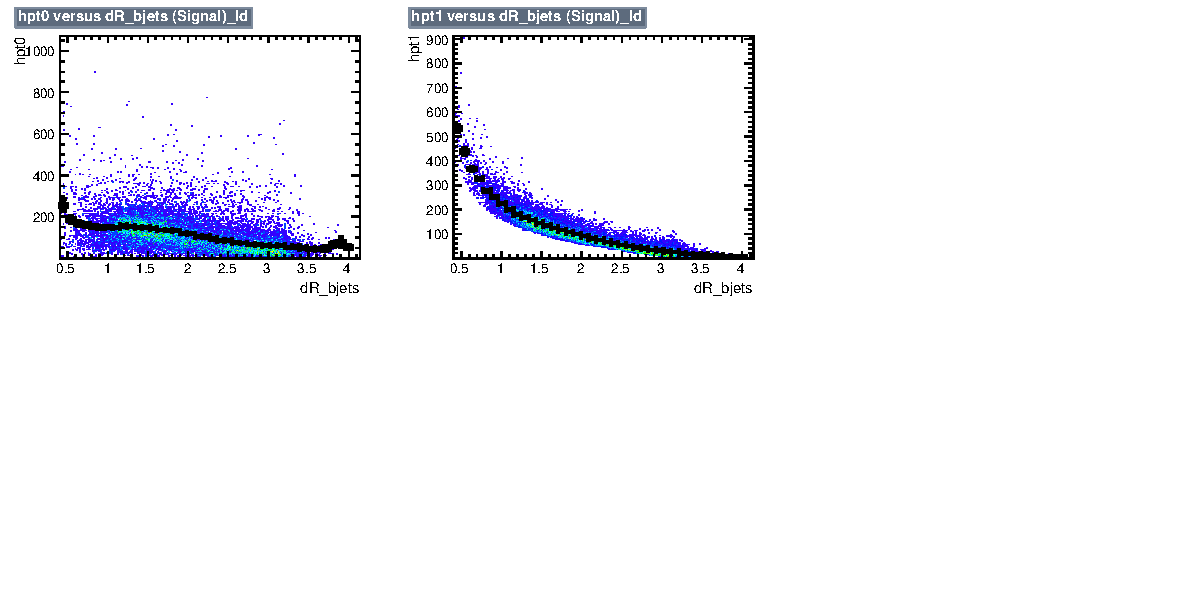
\includegraphics[width=0.95\textwidth]{figures/SR/dataset/plots/correlationscatter_dR_bjets__Id_c2.pdf}
\caption{ Correlation scatter plots for dR between bjets variable for signal}%, index '1' refers to bb and index '0' refers to ZZ}
\label{fig:correlations_SR_drbjets_S}                                                       
\end{figure}



\begin{figure}[!htb]%hbpt?        
\centering
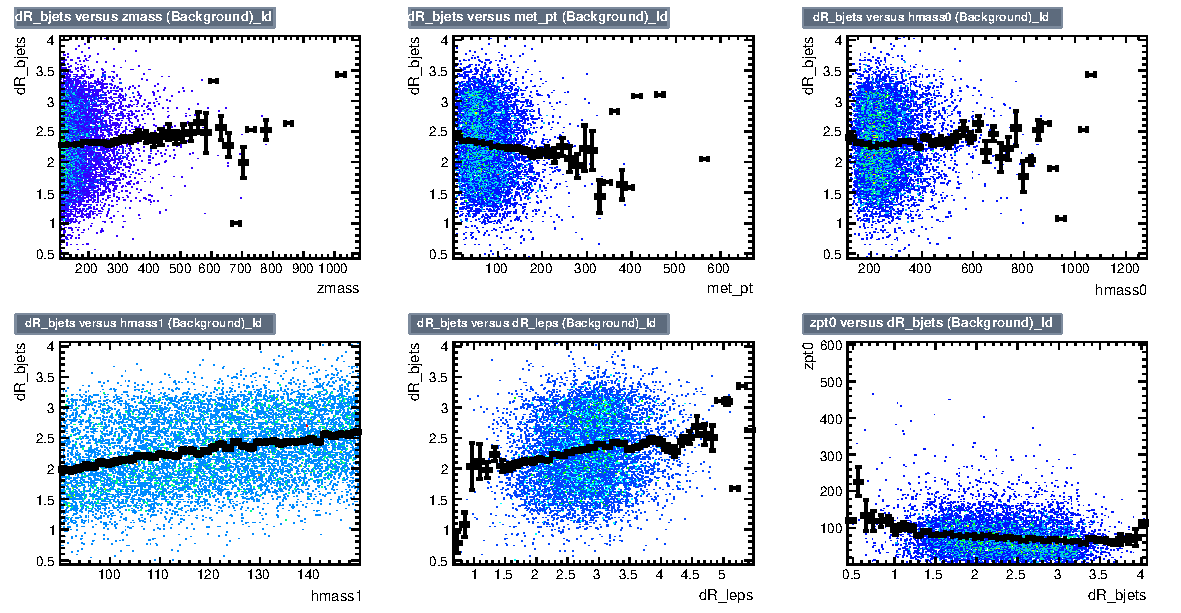
\includegraphics[width=0.95\textwidth]{figures/SR/dataset/plots/correlationscatter_dR_bjets__Id_c3.pdf}
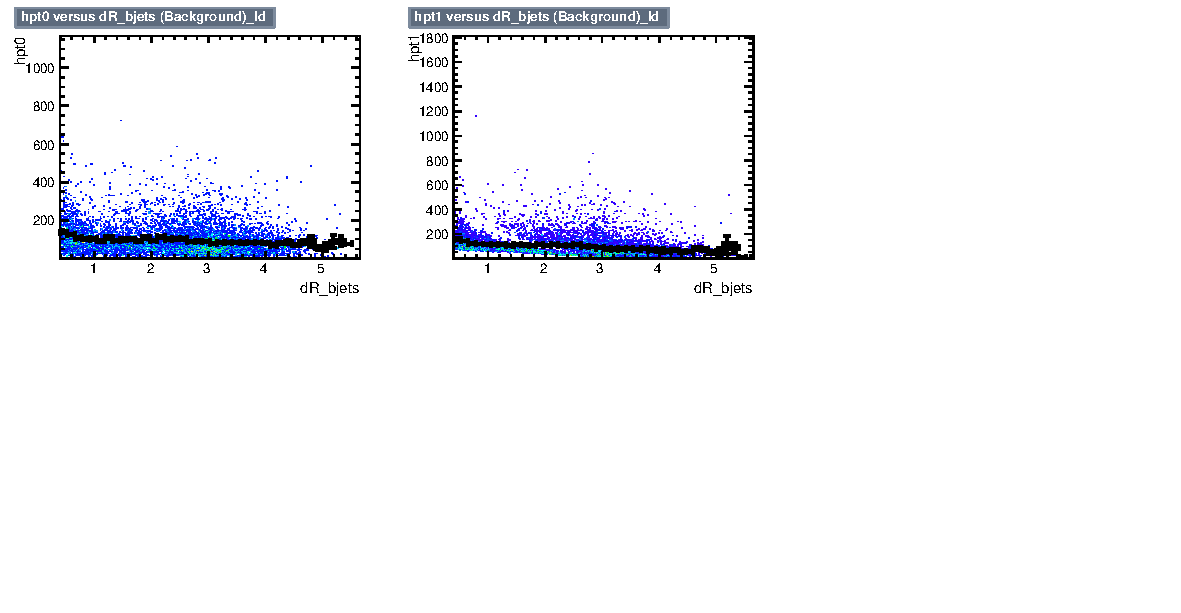
\includegraphics[width=0.95\textwidth]{figures/SR/dataset/plots/correlationscatter_dR_bjets__Id_c4.pdf}
\caption{ Correlation scatter plots for dR between bjets variable for backgrounds}%, index '1' refers to bb and index '0' refers to ZZ}
\label{fig:correlations_SR_drbjets_BG}                                                       
\end{figure}




\begin{figure}[!htb]%hbpt?        
\centering
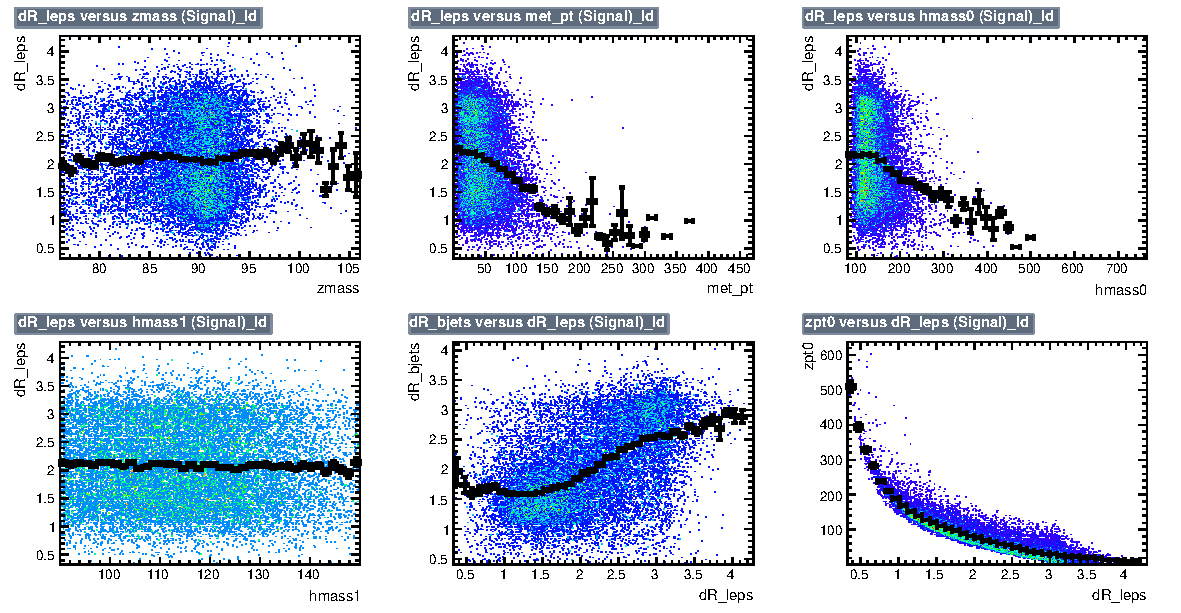
\includegraphics[width=0.95\textwidth]{figures/SR/dataset/plots/correlationscatter_dR_leps__Id_c1.pdf}
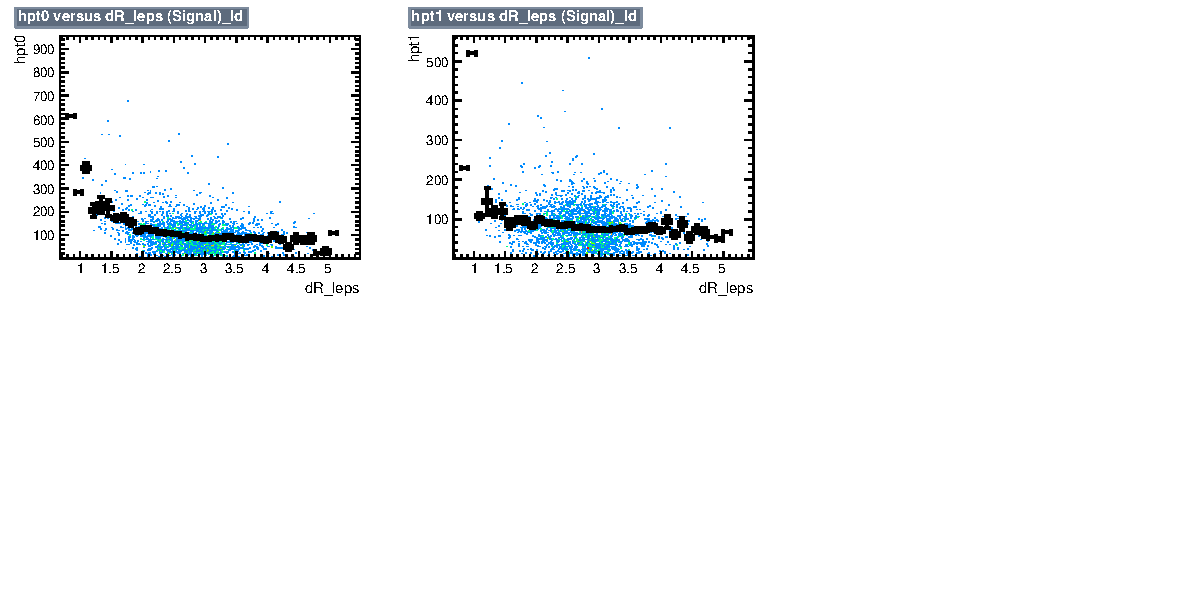
\includegraphics[width=0.95\textwidth]{figures/SR/dataset/plots/correlationscatter_dR_leps__Id_c2.pdf}
\caption{ Correlation scatter plots for dR between leptons variable for signal}%, index '1' refers to bb and index '0' refers to ZZ}
\label{fig:correlations_SR_drleps_S}                                                       
\end{figure}



\begin{figure}[!htb]%hbpt?        
\centering
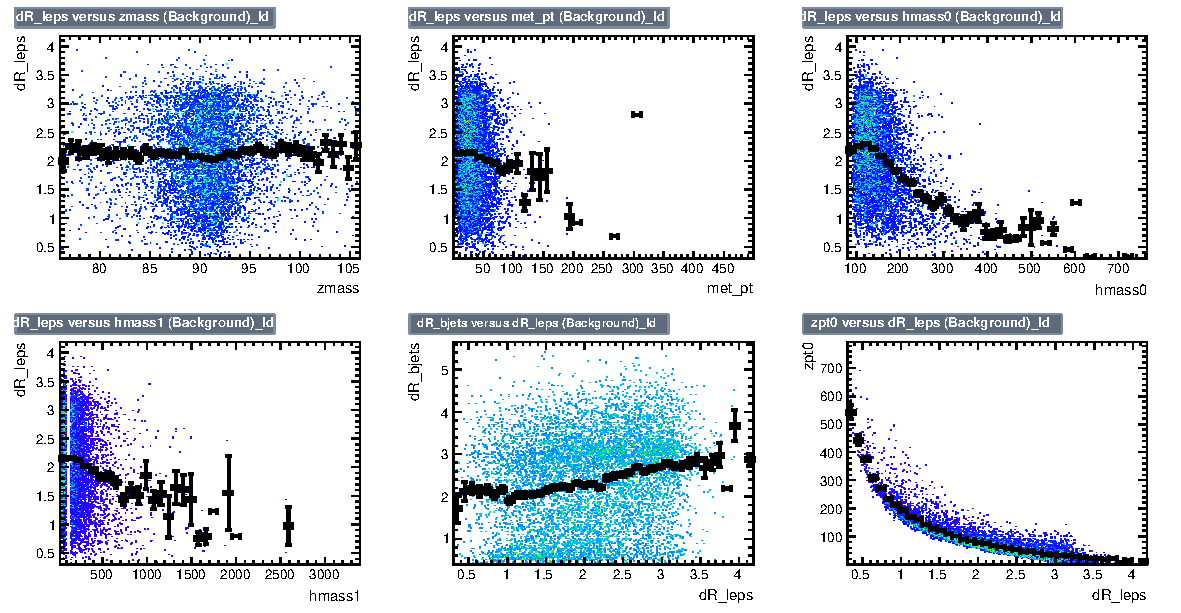
\includegraphics[width=0.95\textwidth]{figures/SR/dataset/plots/correlationscatter_dR_leps__Id_c3.pdf}
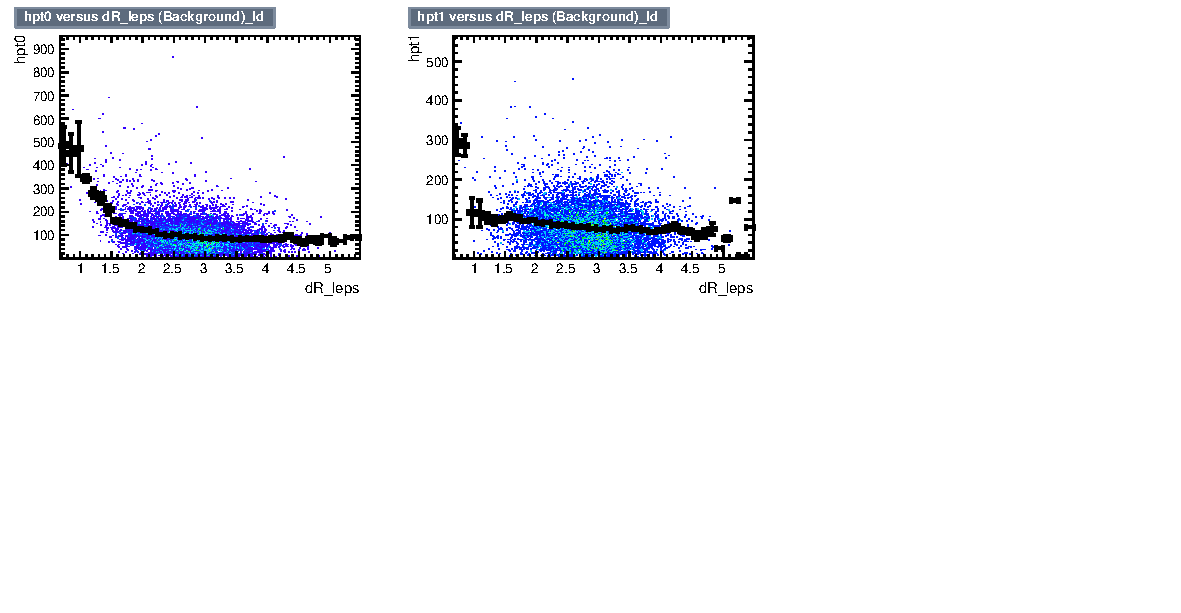
\includegraphics[width=0.95\textwidth]{figures/SR/dataset/plots/correlationscatter_dR_leps__Id_c4.pdf}
\caption{ Correlation scatter plots for dR between keptons variable for backgrounds}%, index '1' refers to bb and index '0' refers to ZZ}
\label{fig:correlations_SR_drleps_BG}                                                       
\end{figure}



\begin{figure}[!htb]%hbpt?        
\centering
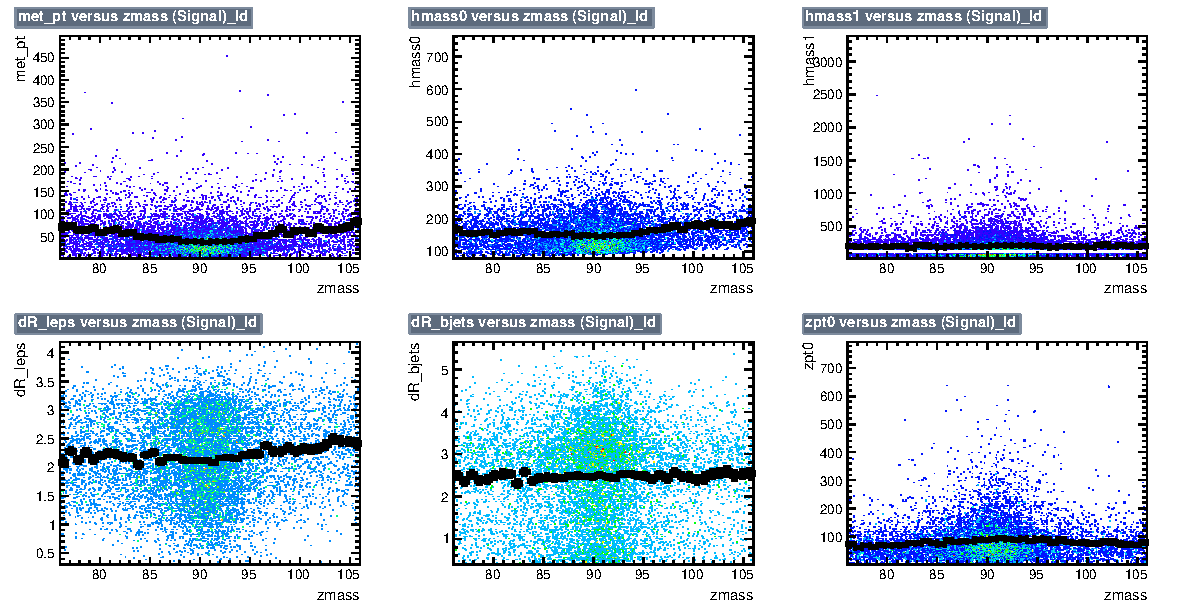
\includegraphics[width=0.95\textwidth]{figures/SR/dataset/plots/correlationscatter_zmass__Id_c1.pdf}
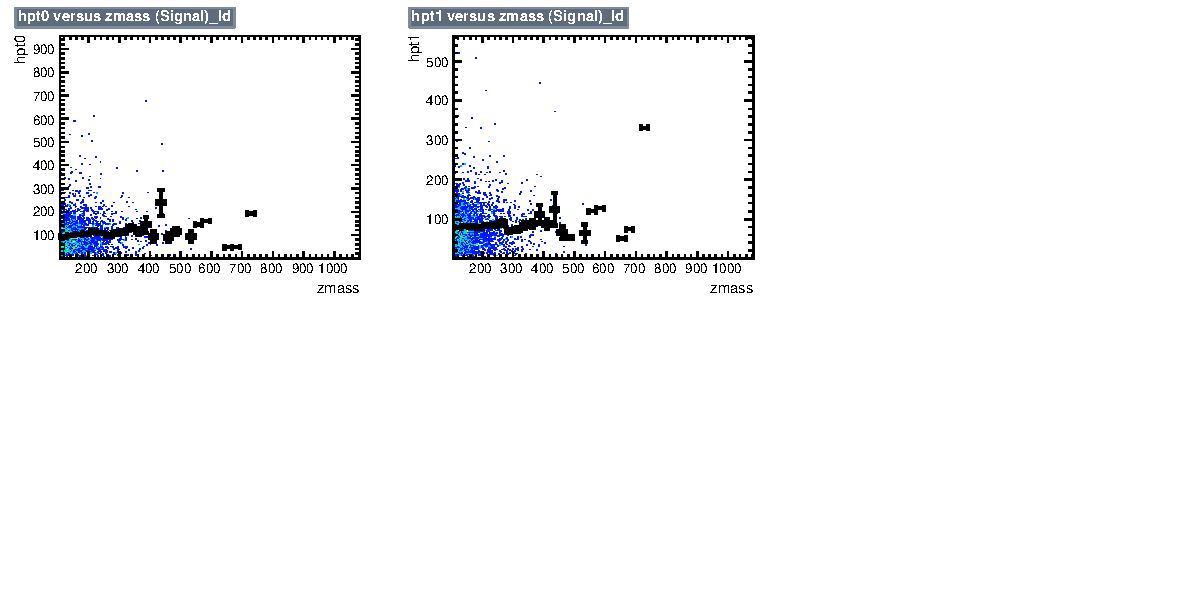
\includegraphics[width=0.95\textwidth]{figures/SR/dataset/plots/correlationscatter_zmass__Id_c2.pdf}
\caption{ Correlation scatter plots for \Zll bjets variable for signal}%, index '1' refers to bb and index '0' refers to ZZ}
\label{fig:correlations_SR_zmass_S}                                                       
\end{figure}



\begin{figure}[!htb]%hbpt?        
\centering
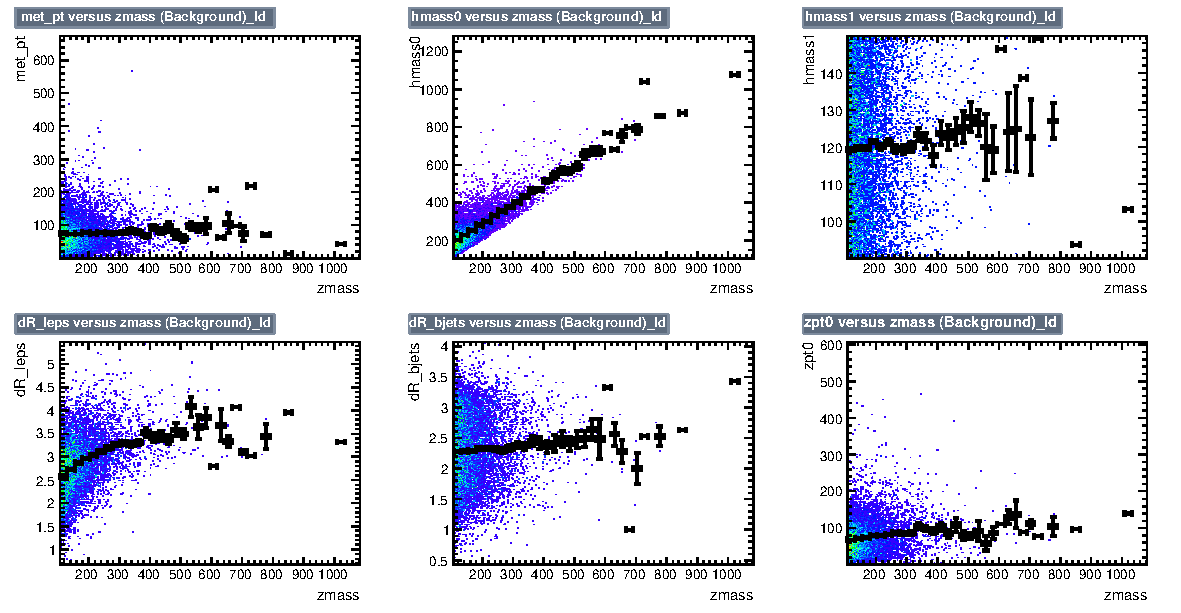
\includegraphics[width=0.95\textwidth]{figures/SR/dataset/plots/correlationscatter_zmass__Id_c3.pdf}
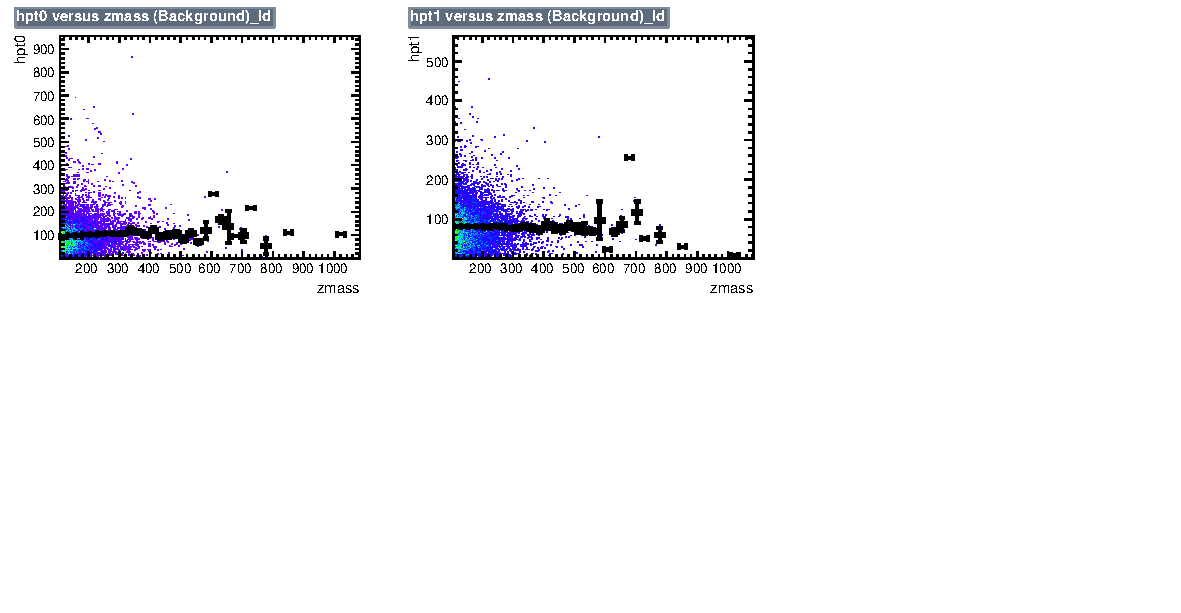
\includegraphics[width=0.95\textwidth]{figures/SR/dataset/plots/correlationscatter_zmass__Id_c4.pdf}
\caption{ Correlation scatter plots for \Zll mass variable for backgrounds}%, index '1' refers to bb and index '0' refers to ZZ}
\label{fig:correlations_SR_zmass_BG}                                                       
\end{figure}



\begin{figure}[!htb]%hbpt?        
\centering
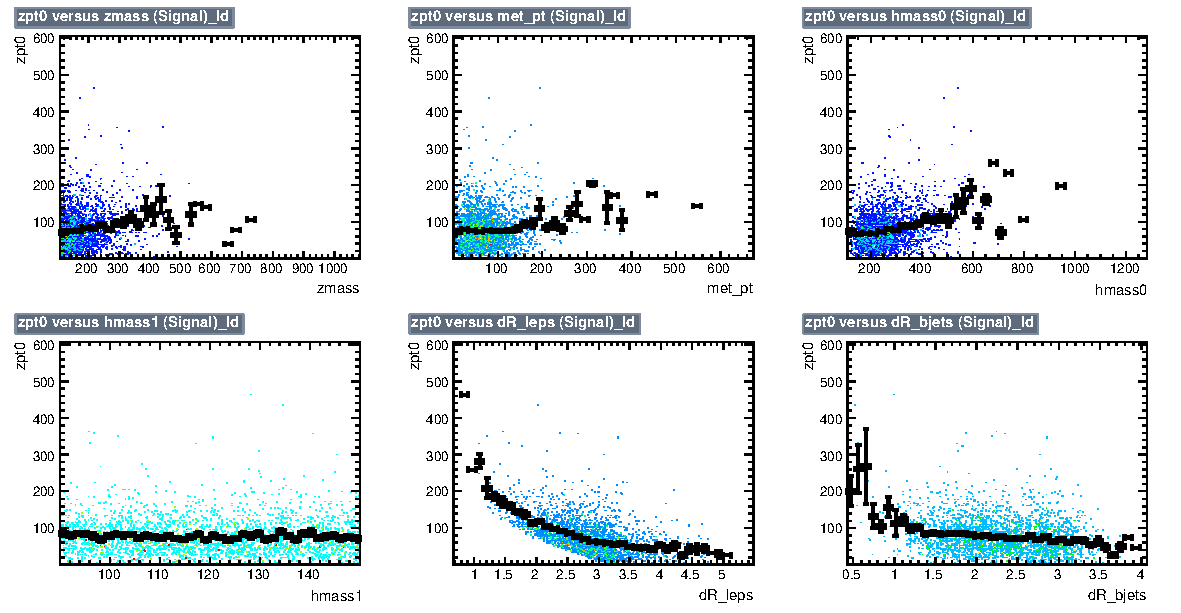
\includegraphics[width=0.95\textwidth]{figures/SR/dataset/plots/correlationscatter_zpt0__Id_c1.pdf}
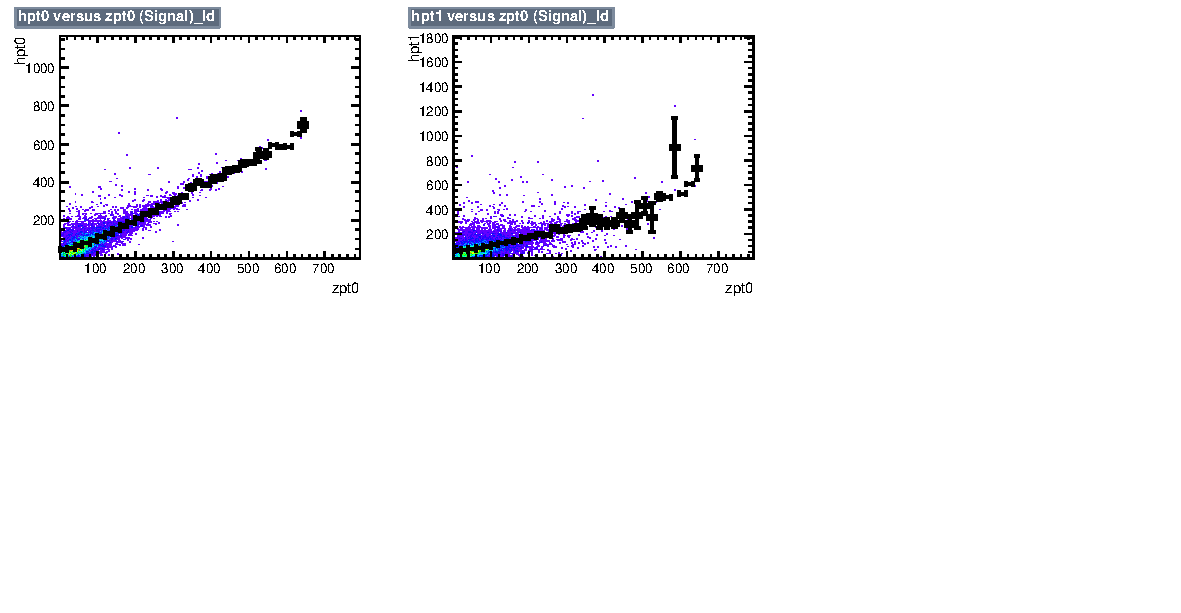
\includegraphics[width=0.95\textwidth]{figures/SR/dataset/plots/correlationscatter_zpt0__Id_c2.pdf}
\caption{ Correlation scatter plots for Z $p_{T}$  variable for signal}%, index '1' refers to bb and index '0' refers to ZZ}
\label{fig:correlations_SR_zpt_S}                                                       
\end{figure}



\begin{figure}[!htb]%hbpt?        
\centering
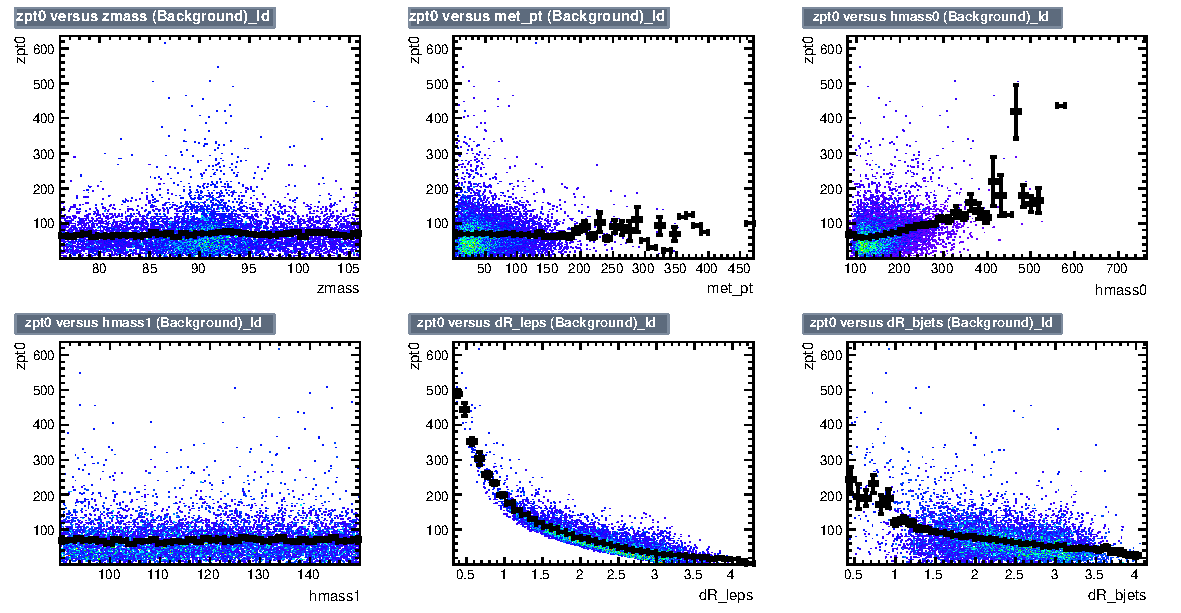
\includegraphics[width=0.95\textwidth]{figures/SR/dataset/plots/correlationscatter_zpt0__Id_c3.pdf}
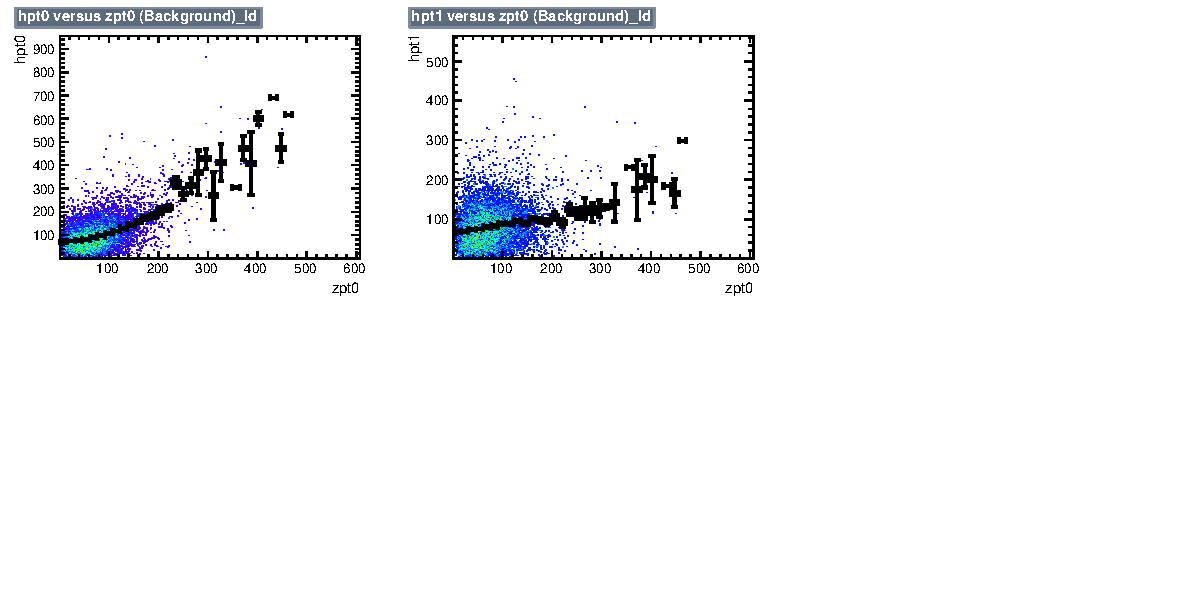
\includegraphics[width=0.95\textwidth]{figures/SR/dataset/plots/correlationscatter_zpt0__Id_c4.pdf}
\caption{ Correlation scatter plots for Z $p_{T}$ variable for backgrounds}%, index '1' refers to bb and index '0' refers to ZZ}
\label{fig:correlations_SR_zpt_BG}                                                       
\end{figure}


\begin{figure}[!htb]%hbpt?        
\centering
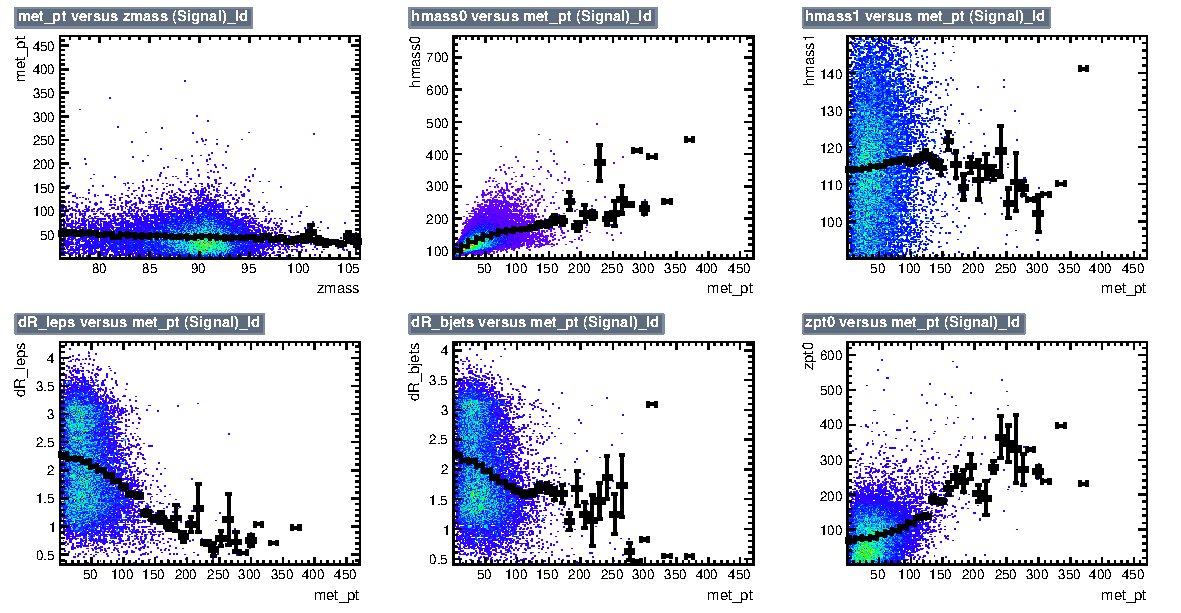
\includegraphics[width=0.95\textwidth]{figures/SR/dataset/plots/correlationscatter_met_pt__Id_c1.pdf}
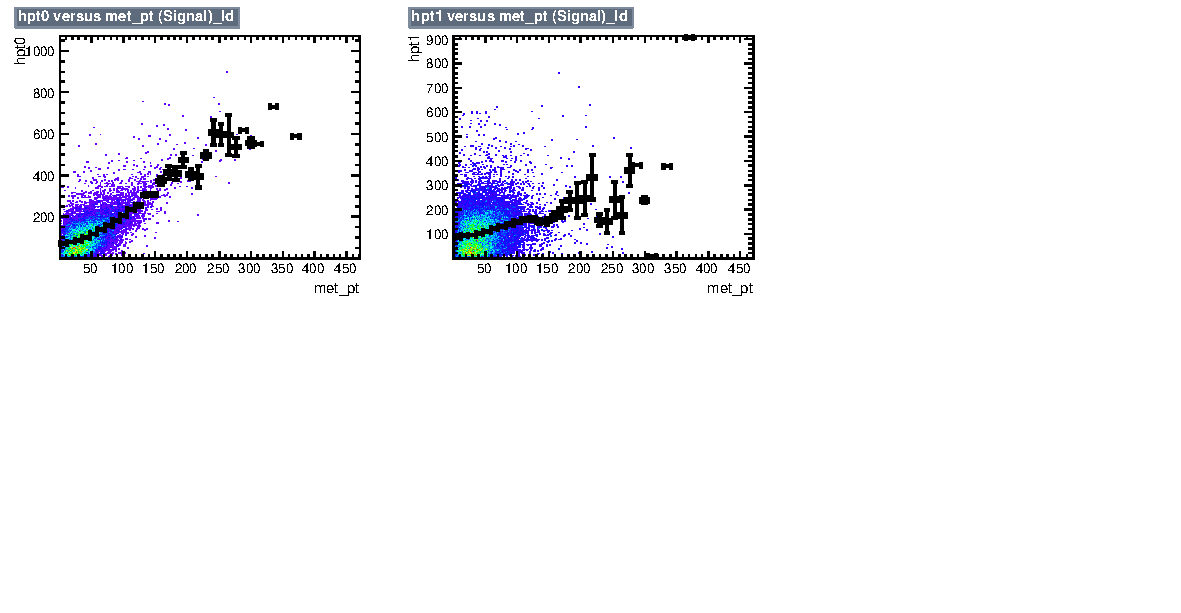
\includegraphics[width=0.95\textwidth]{figures/SR/dataset/plots/correlationscatter_met_pt__Id_c2.pdf}
\caption{ Correlation scatter plots for met variable for signal}%, index '1' refers to bb and index '0' refers to ZZ}
\label{fig:correlations_SR_met_pt_S}                                                       
\end{figure}



\begin{figure}[!htb]%hbpt?        
\centering
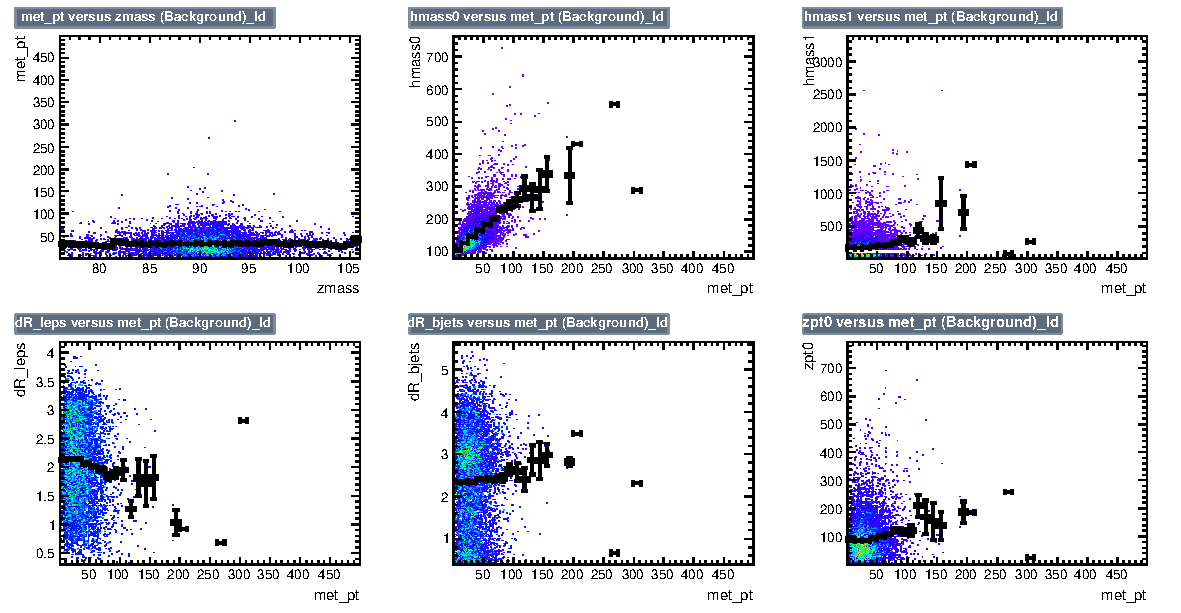
\includegraphics[width=0.95\textwidth]{figures/SR/dataset/plots/correlationscatter_met_pt__Id_c3.pdf}
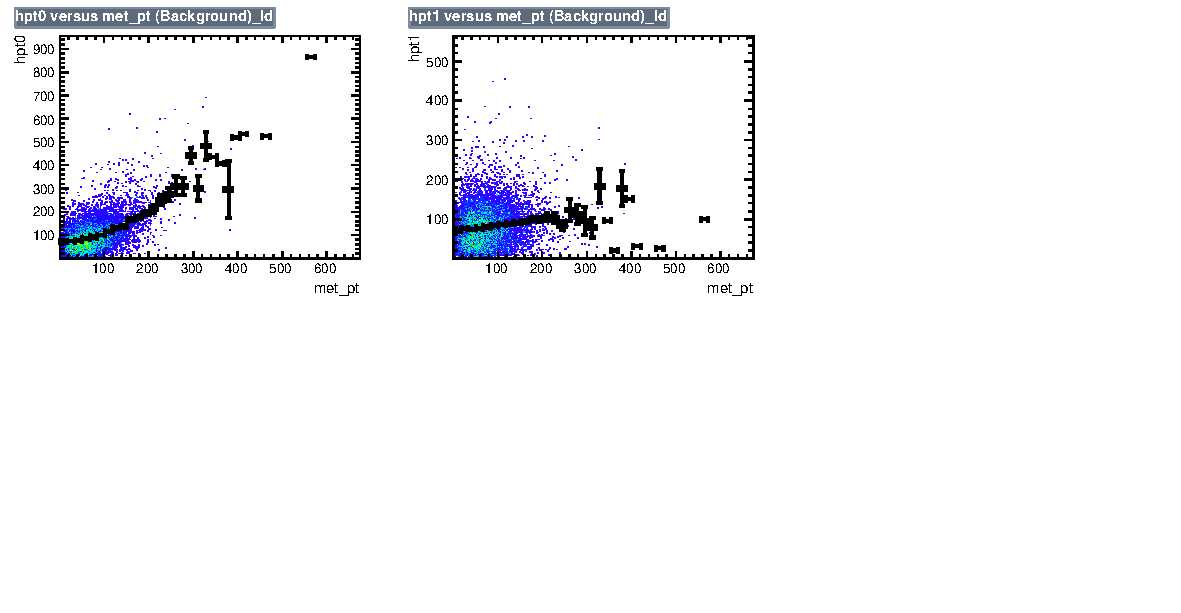
\includegraphics[width=0.95\textwidth]{figures/SR/dataset/plots/correlationscatter_met_pt__Id_c4.pdf}
\caption{ Correlation scatter plots for met variable for backgrounds}%, index '1' refers to bb and index '0' refers to ZZ}
\label{fig:correlations_SR_met_pt_BG}                                                       
\end{figure}





\begin{figure}[!htb]%hbpt?        
\centering
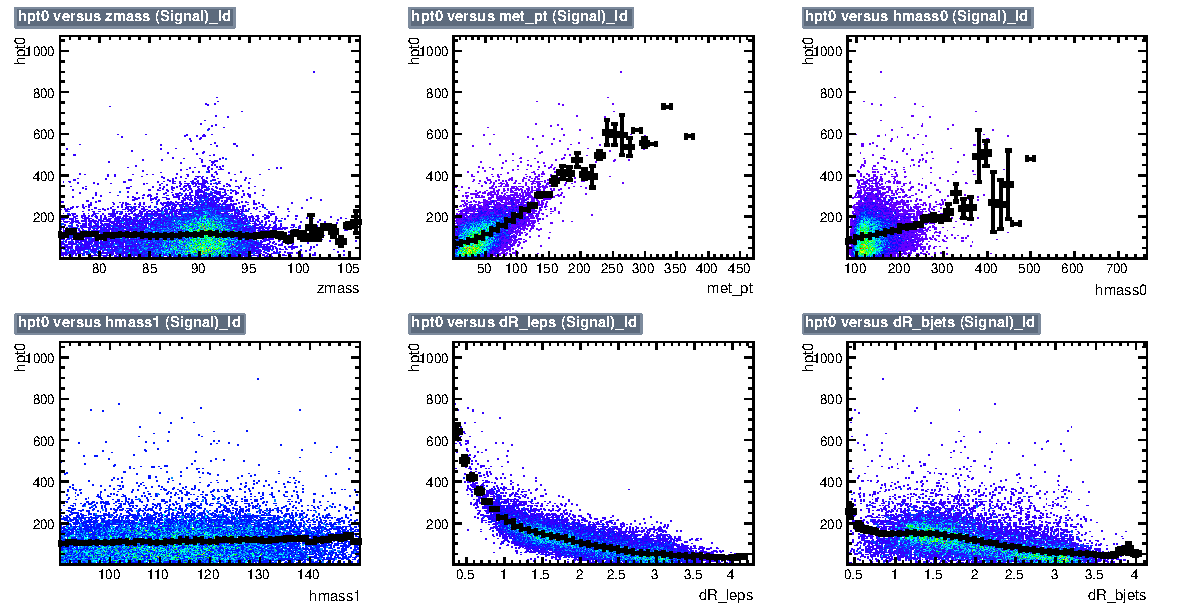
\includegraphics[width=0.95\textwidth]{figures/SR/dataset/plots/correlationscatter_hpt0__Id_c1.pdf}
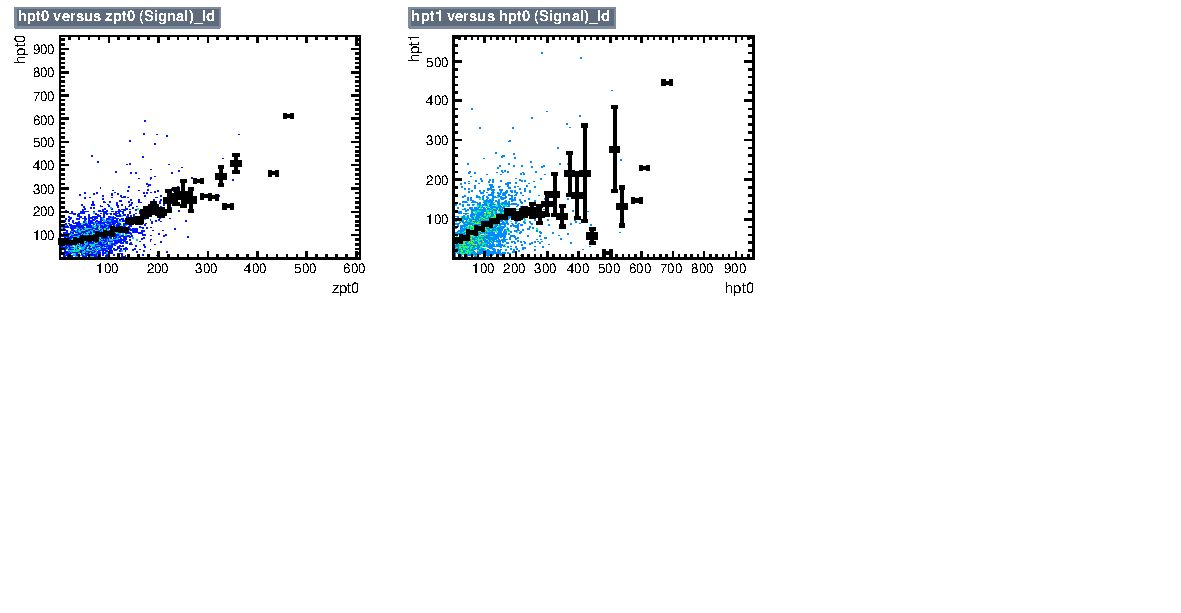
\includegraphics[width=0.95\textwidth]{figures/SR/dataset/plots/correlationscatter_hpt0__Id_c2.pdf}
\caption{ Correlation scatter plots for \HZZ $p_{T}$  variable for signal}%, index '1' refers to bb and index '0' refers to ZZ}
\label{fig:correlations_SR_hpt0_S}                                                       
\end{figure}



\begin{figure}[!htb]%hbpt?        
\centering
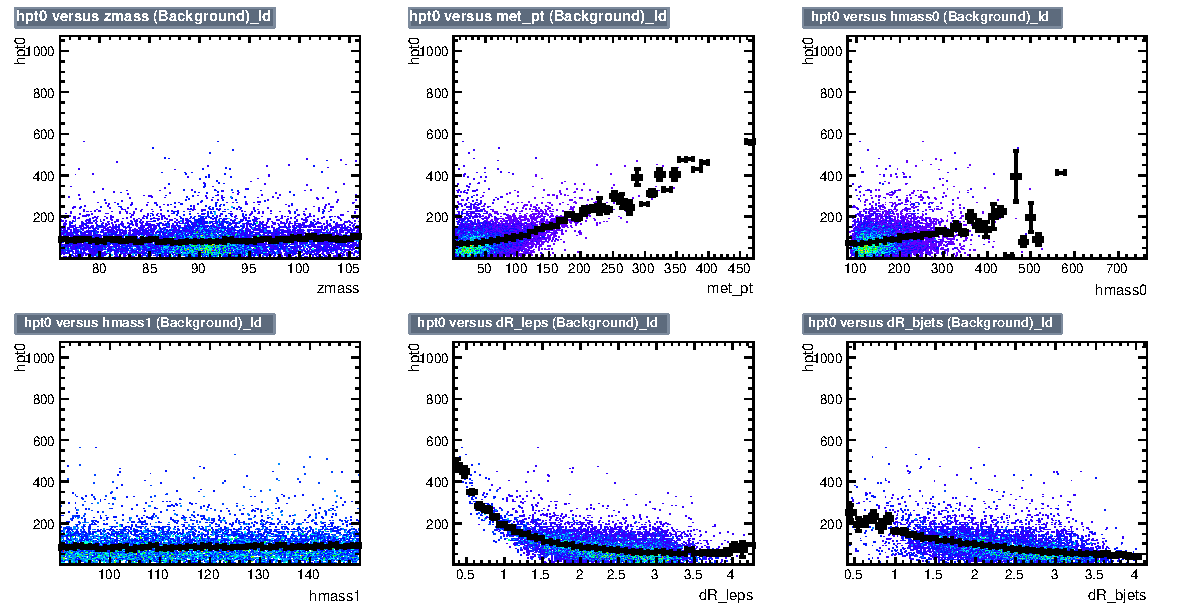
\includegraphics[width=0.95\textwidth]{figures/SR/dataset/plots/correlationscatter_hpt0__Id_c3.pdf}
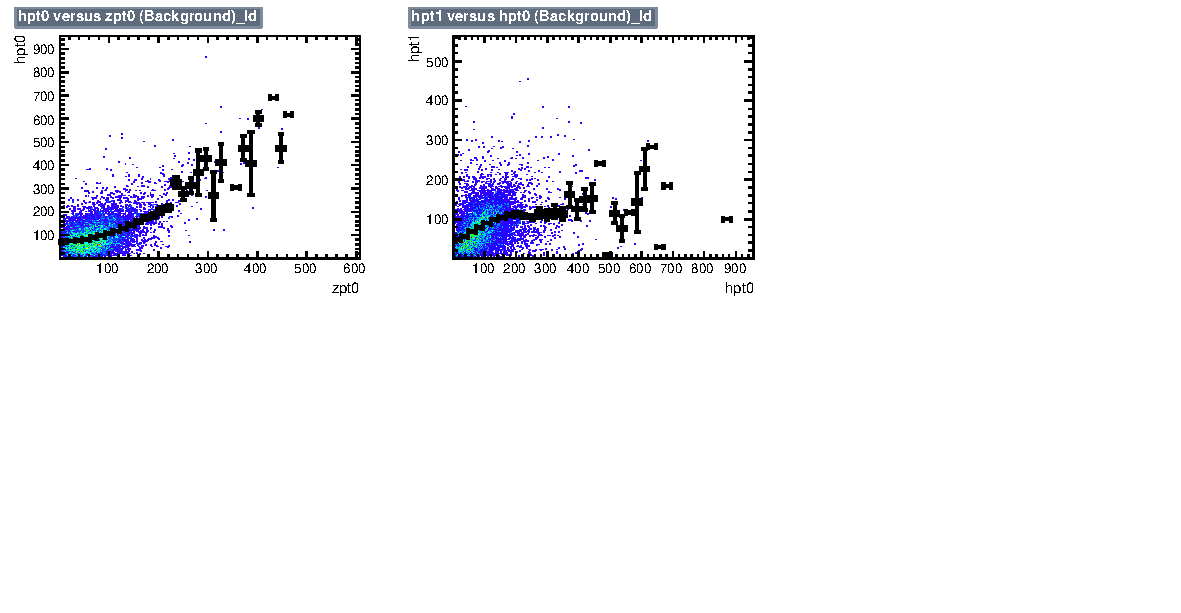
\includegraphics[width=0.95\textwidth]{figures/SR/dataset/plots/correlationscatter_hpt0__Id_c4.pdf}
\caption{ Correlation scatter plots for \HZZ $p_{T}$ variable for backgrounds}%, index '1' refers to bb and index '0' refers to ZZ}
\label{fig:correlations_SR_hpt0_BG}                                                       
\end{figure}


\begin{figure}[!htb]%hbpt?        
\centering
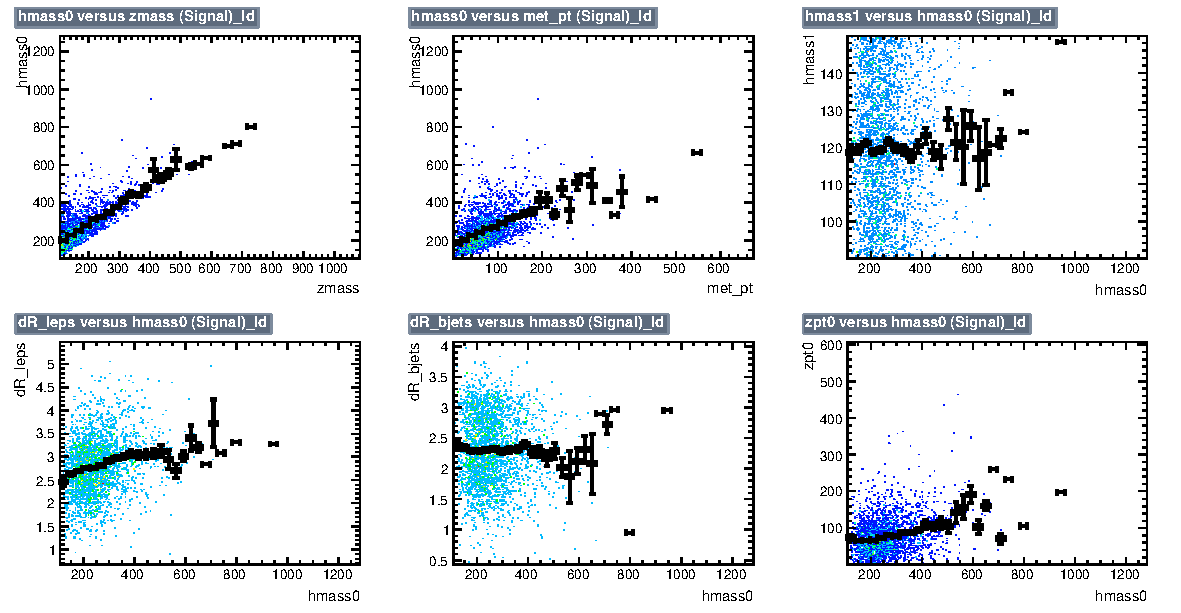
\includegraphics[width=0.95\textwidth]{figures/SR/dataset/plots/correlationscatter_hmass0__Id_c1.pdf}
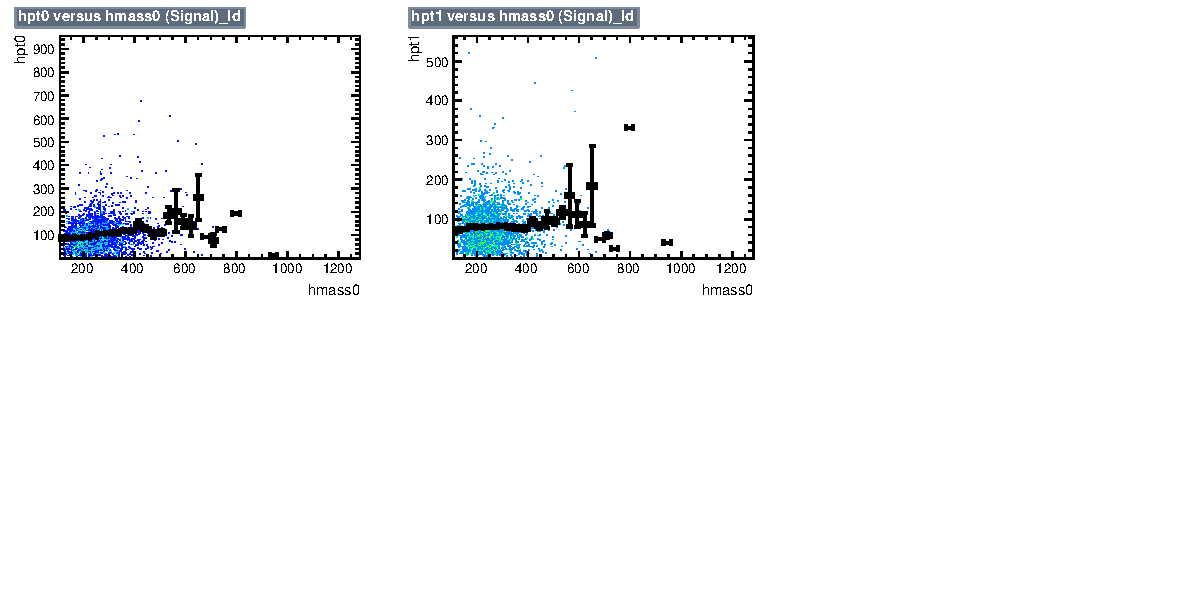
\includegraphics[width=0.95\textwidth]{figures/SR/dataset/plots/correlationscatter_hmass0__Id_c2.pdf}
\caption{ Correlation scatter plots for \HZZ mass  variable for signal}%, index '1' refers to bb and index '0' refers to ZZ}
\label{fig:correlations_SR_hmass0_S}                                                       
\end{figure}



\begin{figure}[!htb]%hbpt?        
\centering
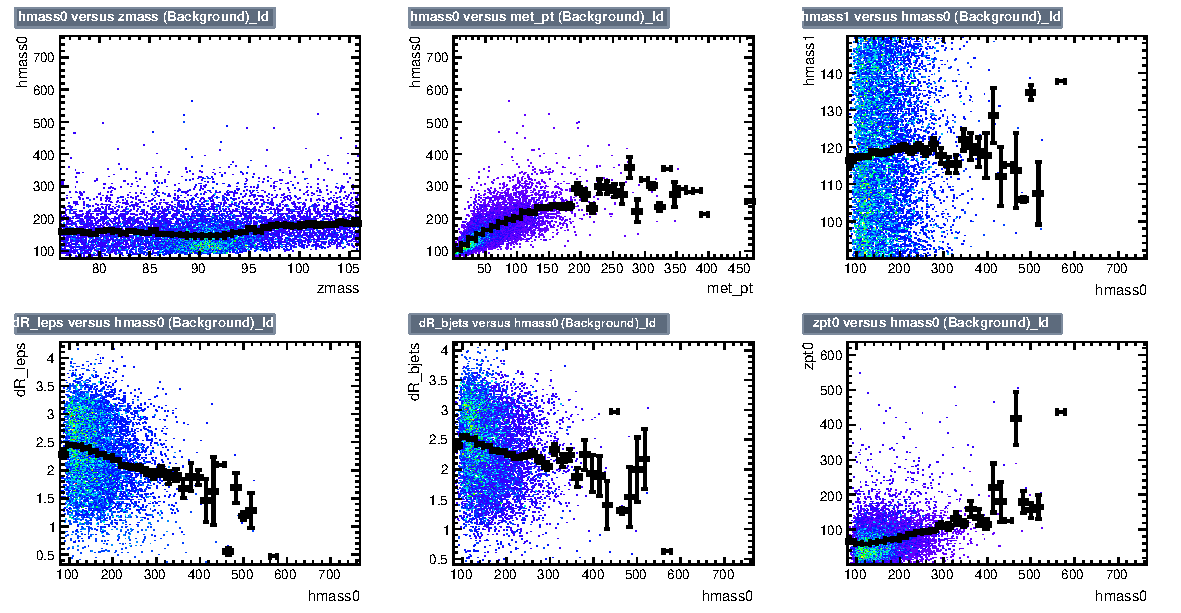
\includegraphics[width=0.95\textwidth]{figures/SR/dataset/plots/correlationscatter_hmass0__Id_c3.pdf}
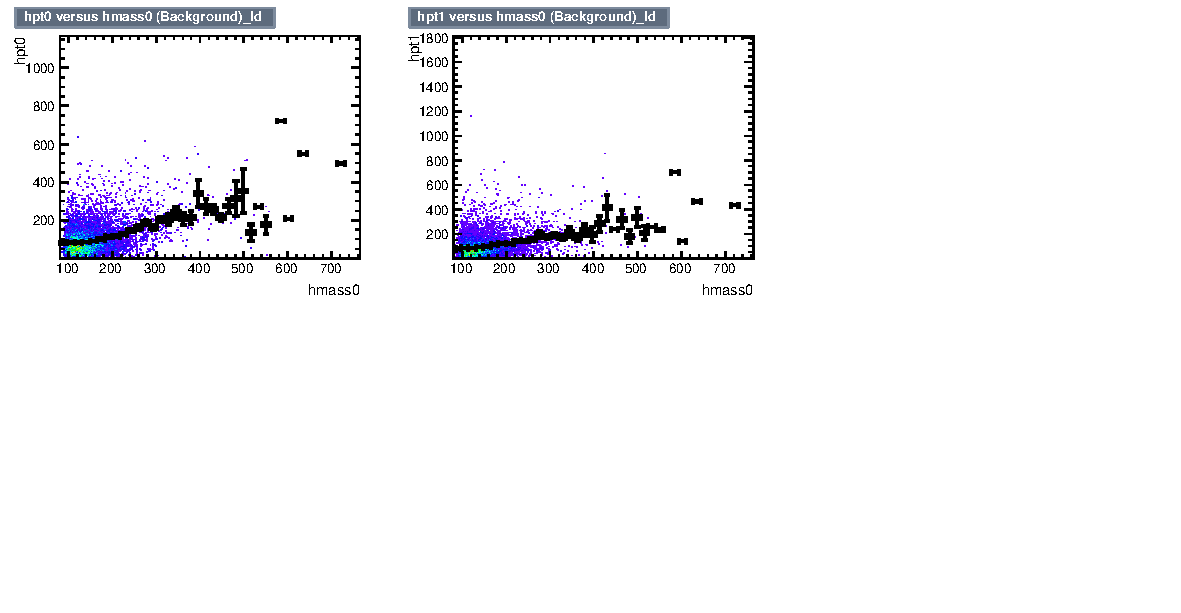
\includegraphics[width=0.95\textwidth]{figures/SR/dataset/plots/correlationscatter_hmass0__Id_c4.pdf}
\caption{ Correlation scatter plots for \HZZ mass variable for backgrounds}%, index '1' refers to bb and index '0' refers to ZZ}
\label{fig:correlations_SR_hmass0_BG}                                                       
\end{figure}




\begin{figure}[!htb]%hbpt?        
\centering
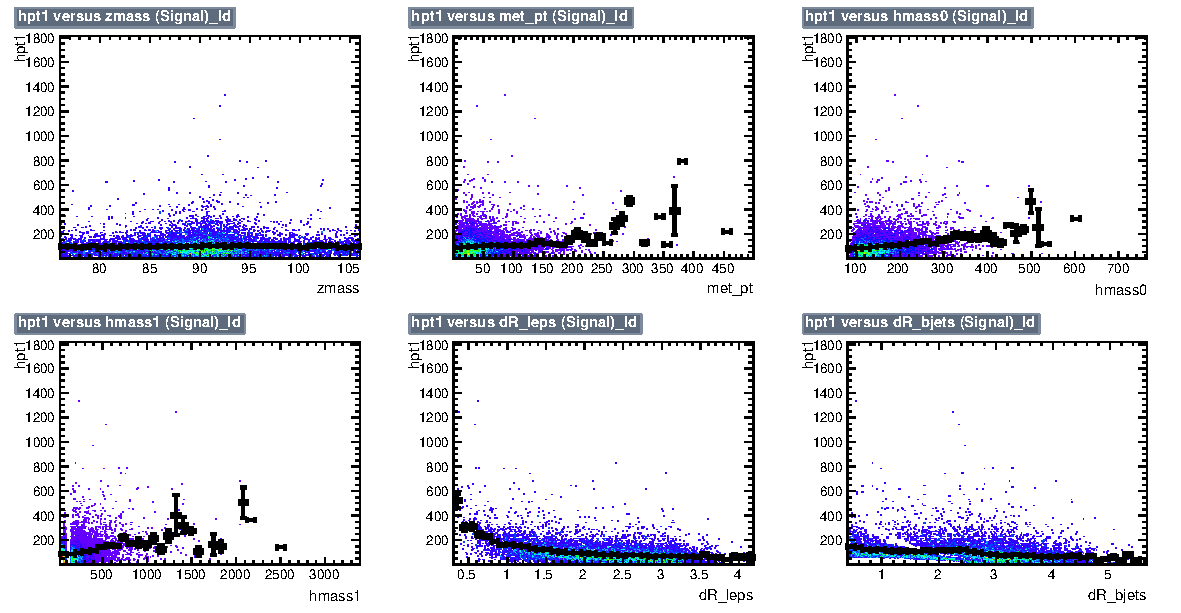
\includegraphics[width=0.95\textwidth]{figures/SR/dataset/plots/correlationscatter_hpt1__Id_c1.pdf}
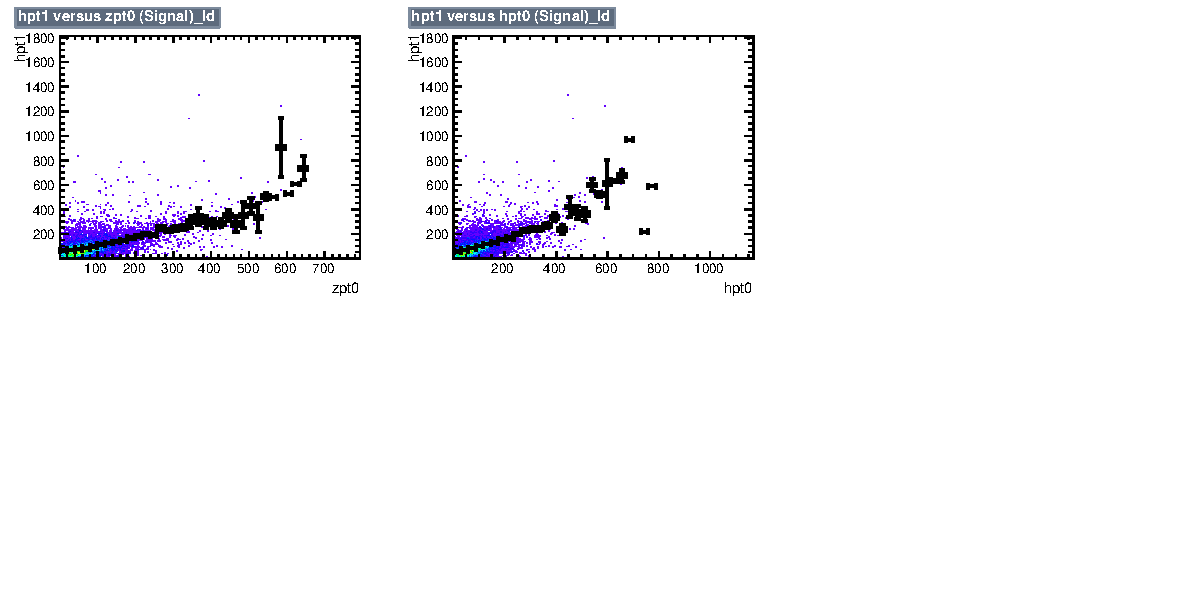
\includegraphics[width=0.95\textwidth]{figures/SR/dataset/plots/correlationscatter_hpt1__Id_c2.pdf}
\caption{ Correlation scatter plots for \HBB $p_{T}$  variable for signal}%, index '1' refers to bb and index '0' refers to ZZ}
\label{fig:correlations_SR_hpt1_S}                                                       
\end{figure}



\begin{figure}[!htb]%hbpt?        
\centering
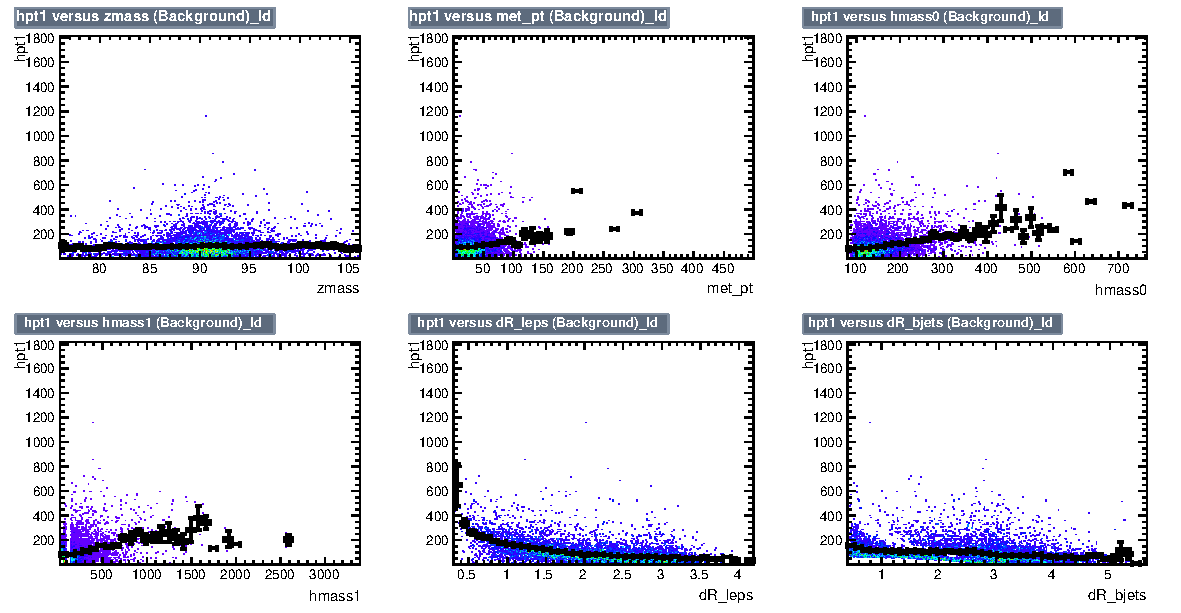
\includegraphics[width=0.95\textwidth]{figures/SR/dataset/plots/correlationscatter_hpt1__Id_c3.pdf}
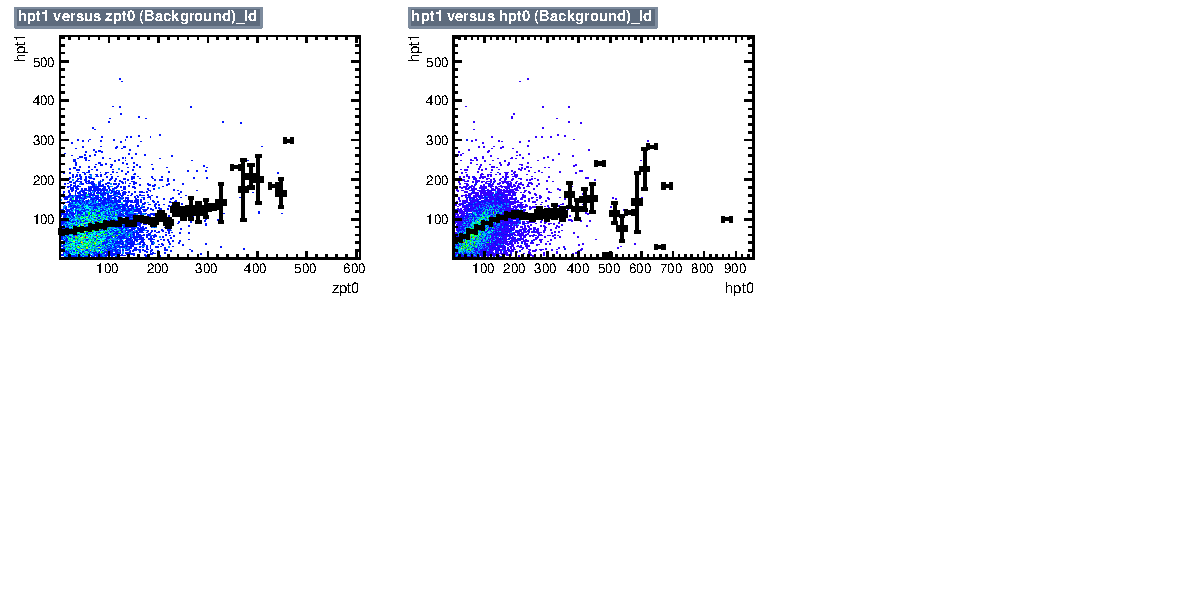
\includegraphics[width=0.95\textwidth]{figures/SR/dataset/plots/correlationscatter_hpt1__Id_c4.pdf}
\caption{ Correlation scatter plots for \HBB $p_{T}$ variable for backgrounds}%, index '1' refers to bb and index '0' refers to ZZ}
\label{fig:correlations_SR_hpt1_BG}                                                       
\end{figure}



\begin{figure}[!htb]%hbpt?        
\centering
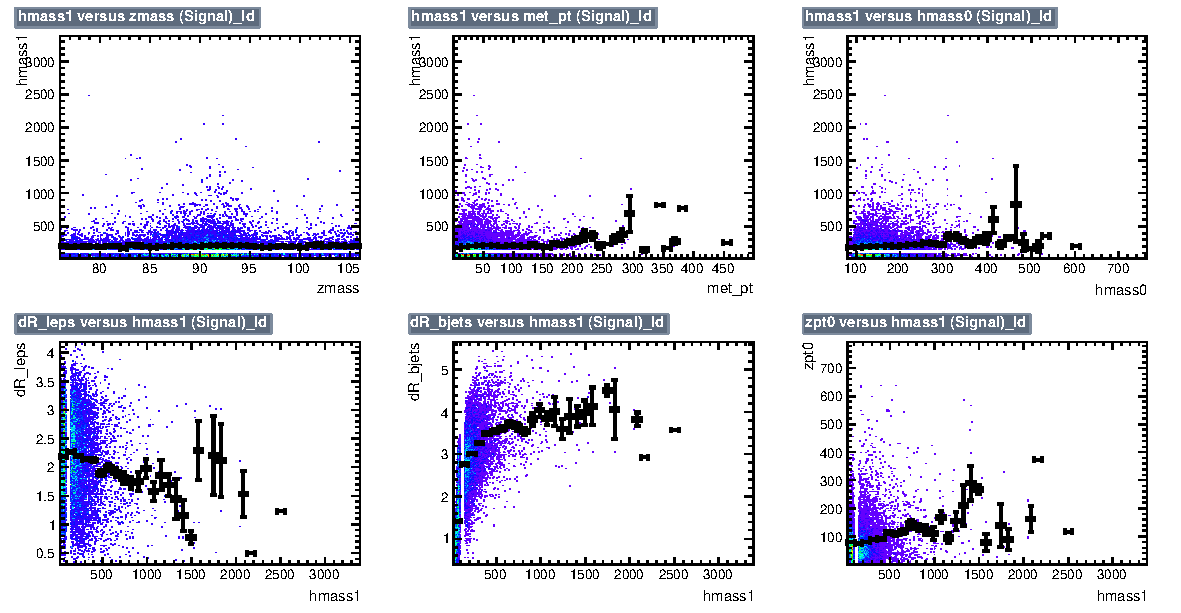
\includegraphics[width=0.95\textwidth]{figures/SR/dataset/plots/correlationscatter_hmass1__Id_c1.pdf}
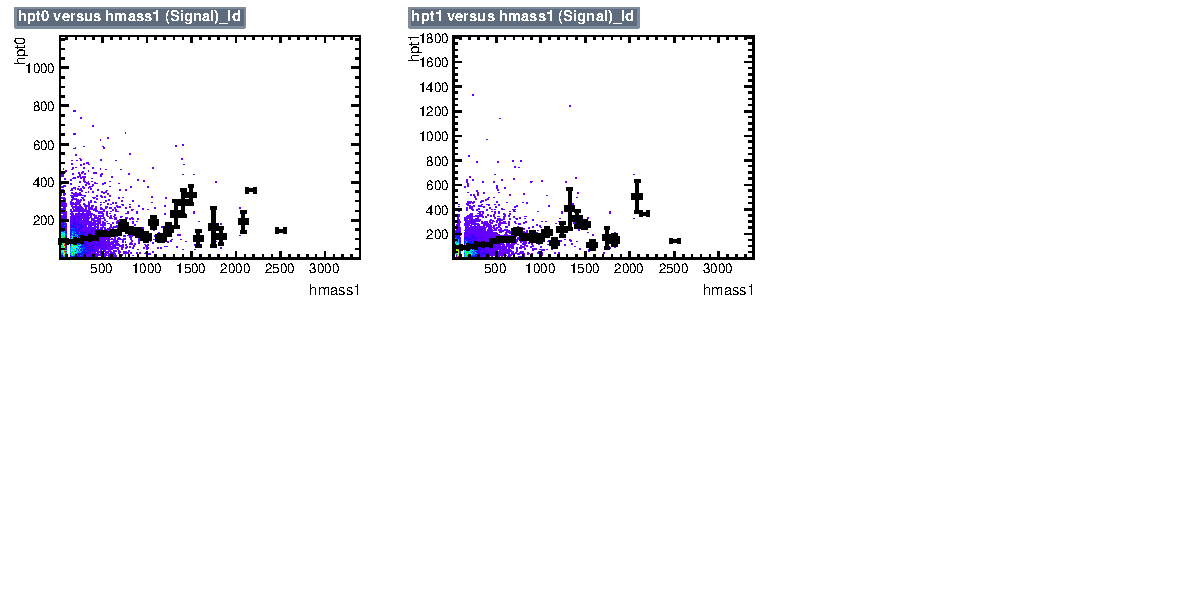
\includegraphics[width=0.95\textwidth]{figures/SR/dataset/plots/correlationscatter_hmass1__Id_c2.pdf}
\caption{ Correlation scatter plots for \HBB mass  variable for signal}%, index '1' refers to bb and index '0' refers to ZZ}
\label{fig:correlations_SR_hmass1_S}                                                       
\end{figure}


%%%%%%    causes 
%! Undefined control sequence. \caption@ORI@xfloat ... \global \setbox \@currbox \color@vbox \normalcolor \... l.204 \begin{figure}[!htb]
\begin{figure}[!htb]%hbpt?        
\centering
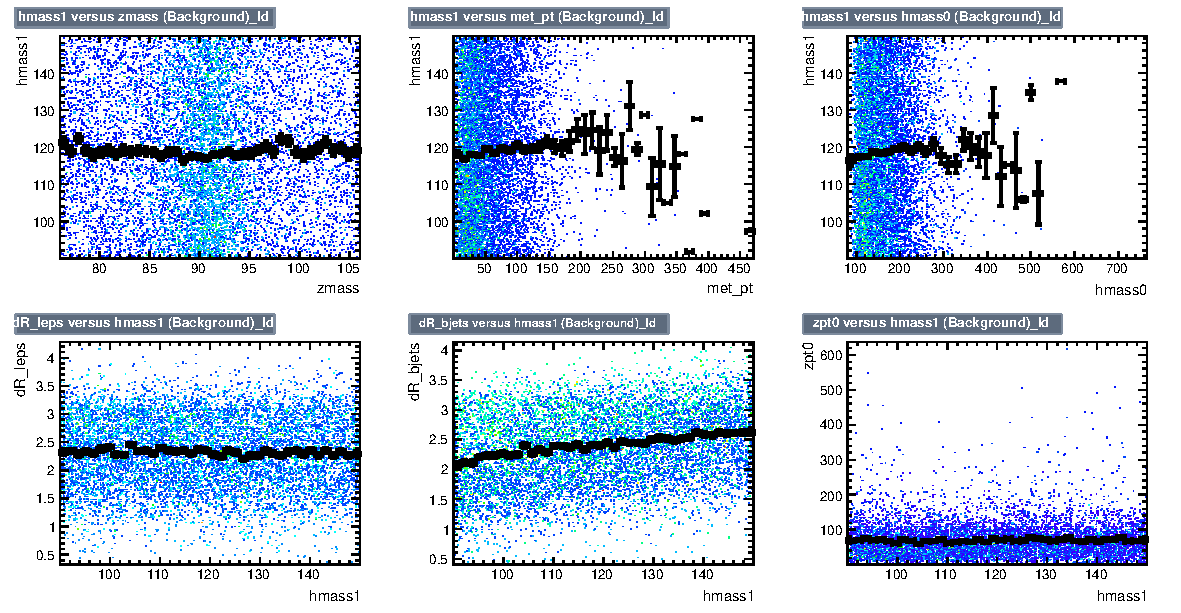
\includegraphics[width=0.95\textwidth]{figures/SR/dataset/plots/correlationscatter_hmass1__Id_c3.pdf}
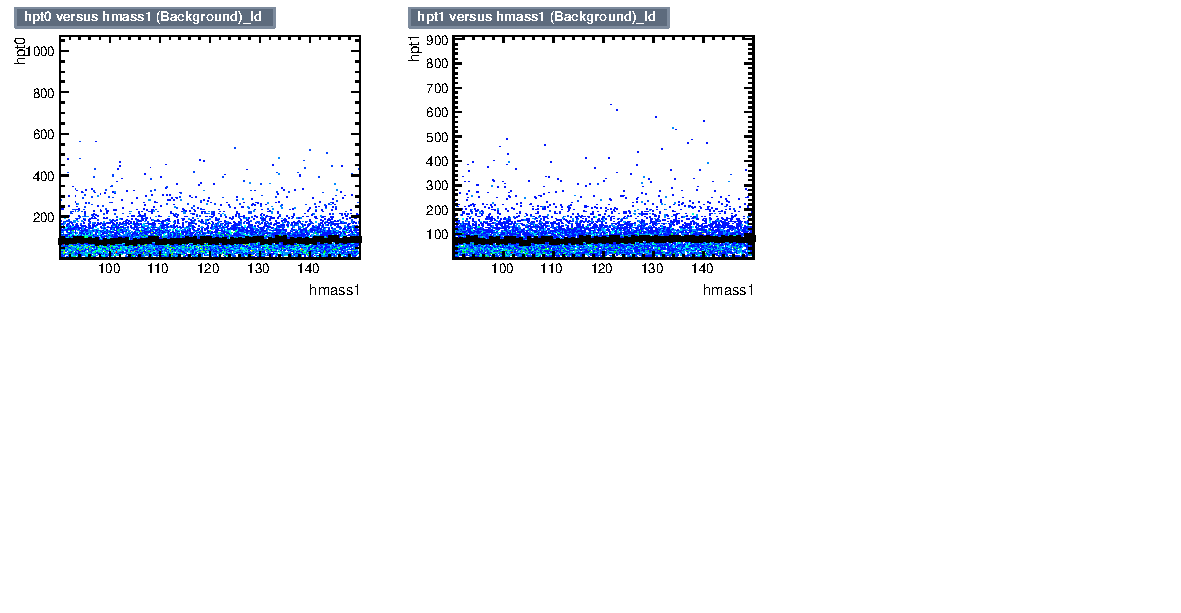
\includegraphics[width=0.95\textwidth]{figures/SR/dataset/plots/correlationscatter_hmass1__Id_c4.pdf}
\caption{ Correlation scatter plots for \HBB mass variable for backgrounds}%, index '1' refers to bb and index '0' refers to ZZ}
\label{fig:correlations_SR_hmass1_BG}                                                       
\end{figure}
 

